
\newvideofile{Netzwerke}{Einfache Widerstandsnetzwerke}

\section{Einfache Widerstandsnetzwerke}




\begin{frame}{}
	\s{
	
		Elektrische Netzwerke setzen sich häufig aus einfacheren Teilschaltungen zusammen. Oft ist es hilfreich, diese Teilschaltungen 
		zu identifizieren, zu vereinfachen und anschließend zur Gesamtschaltung zusammenzufassen. Solche Zusammenfassungen von Bauelementen
		sind grundsätzlich zulässig, sofern sich das \textbf{Klemmverhalten}, also das Verhalten zwischen Strom und Spannung 
		zwischen den Anschlusspunkten, nicht ändert. 
	}
	
	
	
	\ftx{Lernziele: Einfache Gleichstromsnetzwerke}
	
	\begin{Lernziele}{Einfache Widerstandsnetzwerke}
		Die Studierenden können
		\begin{itemize}
			\item Teilschaltungen in gleichstromnetzwerken identifizieren
			\item Widerstandsnetzwerke vereinfachen und zusammenfassen
			\item Kurzschluss- sowie Leerlaufdaten bestimmen
			\item Überlagerungsverfahren anwenden
		\end{itemize}
	\end{Lernziele}
	
	\speech{folie15}{1}{Im vorangegangenen Video wurden die Kirchhoffschen Regeln eingeführt.
		Jetzt wollen wir sie auf einfache Gleichstromnetzwerke anwenden, und uns diese Netzwerke dabei ein wenig genauer ansehen.
		Oft lassen sich diese Netzwerke in einfachere Teilschaltungen zerlegen und einzeln analysieren, was den Prozess vereinfacht. 
		Nach diesem Kapitel solltet ihr also in der Lage sein, diese Teilschaltungen in Gleichstromnetzwerken zu identifizieren, die Netzwerke daraufhin zu vereinfachen, und anschließend wieder zusammenzufassen.
		Außerdem werden wir uns mit Kurzschluss- sowie Leerlaufversuchen beschäftigen, und Methoden zur Netzwerkberechnung wie das Überlagerungsverfahren kennen lernen.
	}
	
\end{frame}







\begin{frame}
	\ftx{Reihenschaltung von Widerständen}
	
	\s{
	
		\subsection{Reihenschaltung von Widerständen}
		
		In einer Reihenschaltung werden alle Bauelemente vom gleichen Strom $I$ durchflossen 
		(siehe Abbildung \ref{fig:reihenschaltung}). 
		
		
		\begin{figure}[h!]
			\begin{center}
				\begin{tikzpicture}
    \draw(0,0)
    to[short](3,0)
    to[short](3,0.5)

    to[R ,i ,v< , name =R1  , l =$R_1$] (3,2.5)
    to[short](3,3)
    to[short](2.5,3)
    to[R ,i ,v< , name =R2  , l =$R_2$]  (0.5,3)
    to[short](0,3)
    to[short, i<_ , name = i_0](0,2.5)
    to[V, v, i, name=V1] (0,0.5)
    to[short](0,0);

    \varrmore{R1}{$U_1$};
    \varrmore{R2}{$U_2$};
    \varrmore{V1}{$U_0$};
    \iarrmore{V1}{$I$};
\end{tikzpicture}
				\caption{Reihenschaltung von zwei Widerständen und einer Spannungsquelle}
				
				\label{fig:reihenschaltung}
			\end{center}
		\end{figure}
		
		Das Anwenden der Maschenregel (hier: Umlaufrichtung gegen den Uhrzeigersinn) führt zu folgender Maschengleichnung:
		
		\begin{equation*}
			U_0 - U_1 - U_2 =0 
		\end{equation*}
		
		Mit Hilfe des Ohmschen Gesetzes können die Teilspannungen $U_1$ und $U_2$ als Produkt aus Stromstärke und Widerstand dargestellt werden:
		
		
		\begin{equation*}
			U_0 - R_1 \cdot I - R_2 \cdot I = 0
		\end{equation*}
		\begin{equation*}
			U_0 - (R_1+R_2) \cdot I = 0
		\end{equation*}
		
		Die Widerstände $R_1$ und $R_2$ lassen sich in diesem Beispiel durch Addition ihrer Widerstandswerte
		zu $R_1 + R_2 = R_\mathrm{ges}$ zusammenfassen (Abbildung \ref{fig:rges}).
		
		
		\begin{figure}[h!]
			\begin{center}
				\begin{tikzpicture}
				\draw(0,0)
				to[short](3,0) 
				to[short](3,0.5) 
	
				to[R ,i ,v< , name =R1  , l =$R_\mathrm{ges}$] (3,2.5)
				to[short](3,3) 
		%		to[short](2.5,3) 
		%		to[R ,i ,v< , name =R2  , l =$R_2$]  (0.5,3)
				to[short](0,3)
				to[short, i<_ , name = i_0](0,2.5)  
				to[V, v, i, name=V1] (0,0.5)
				to[short](0,0); 
	
			 \varrmore{R1}{$U_\mathrm{ges}$};
		%	 \varrmore{R2}{$U_2$};
			 \varrmore{V1}{$U_0$};		
			 \iarrmore{V1}{$I$};			
			\end{tikzpicture}
				
				\caption{Zusammenfassen von $R_1$ und $R_2$ zu $R_\mathrm{ges}$}
				
				\label{fig:rges}
			\end{center}
		\end{figure}
		
		Allgemein lässt sich die Gesamtspannung $U_\mathrm{ges}$ nach diesem Prinzip folgendermaßen zusammenfassen:
		
		\begin{equation}
			U_\mathrm{ges} = \sum_{k=1}^{n} U_k = \sum_{k=1}^{n} R_k \cdot I = R_\mathrm{ges} \cdot I
			\label{eq:gesamtwiderstand}
		\end{equation}
		
		Ein Koeffizientenvergleich der letzten beiden Terme von Gleichung \ref{eq:gesamtwiderstand} liefert das allgemeingültige 
		Ergebnis, um Widerstände in einer Reihenschaltung zusammenzufassen:
		
		\begin{Merksatz}{Gesamtwiderstand einer Reihenschaltung}{}
			\begin{equation}
				R_\mathrm{ges} = \sum_{k=1}^{n} R_k
			\end{equation}
		\end{Merksatz}
		
		Betrachtet man statt der Widerstandswerte $R$ die Leitwerte $G = 1/R$ der Widerstände, ergibt sich für den Gesamtleitwert
		einer Reihenschaltung: 
		
		
		\begin{Merksatz}{Gesamtleitwert einer Reihenschaltung}{}
			
			
			\begin{equation}
				\frac{1}{G_\mathrm{ges}} = \sum_{k=1}^{n} \frac{1}{G_k}
			\end{equation}
			%	\begin{equation}
			
			%		\frac{1}{G_\mathrm{ges}} = \sum_{k=1}^{n} \frac{1}{G_k}
			
			%	\end{equation}
			
			
		\end{Merksatz}
		
		
		
		
		
		
		%	\begin{equation*}
		
		
		%		U_1 = R_1 \cdot I \quad \quad  U_2 = R_2 \cdot I
		
		%	\end{equation*}
		
		
		
	}
	
	\b{
	
		\begin{columns}


			\column[c]{0.4\textwidth}
			
			\vspace*{-60pt}
			
			Maschenregel:
			
			$U_0 - U_1 - U_2 =0 $\\
			
			\phantom{.}\\
			
			
			
			
			
			Ohmsches Gesetz:
			
			$U_1 = R_1 \cdot I \quad \quad  U_2 = R_2 \cdot I$\\
			
			\phantom{.}\\
			
			
			Der Strom $I$ fließt durch alle Bauelemente:
			
			$U_0 - R_1 \cdot I - R_2 \cdot I = 0$\\
			
			$U_0 - (R_1+R_2) \cdot I = 0$\\
			
			
			
			
			\column[t]{0.3\textwidth}
			\begin{tikzpicture}
				\draw(0,0)
				to[short](3,0) 
				to[short](3,0.5) 
				
				to[R ,i ,v< , name =R1  , l =$R_1$] (3,2.5)
				to[short](3,3) 
				to[short](2.5,3) 
				to[R ,i ,v< , name =R2  , l =$R_2$]  (0.5,3)
				to[short](0,3)
				to[short, i<_ , name = i_0](0,2.5)  
				to[V, v, i, name=V1] (0,0.5)
				to[short](0,0); 
				
				\varrmore{R1}{$U_1$};
				\varrmore{R2}{$U_2$};
				\varrmore{V1}{$U_0$};		
				\iarrmore{V1}{$I$};			
			\end{tikzpicture}
			
			\column[t]{0.3\textwidth}
			\begin{tikzpicture}
				\draw(0,0)
				to[short](3,0) 
				to[short](3,0.5) 
				
				to[R ,i ,v< , name =R1  , l =$R_\mathrm{ges}$] (3,2.5)
				to[short](3,3) 
				%		to[short](2.5,3) 
				%		to[R ,i ,v< , name =R2  , l =$R_2$]  (0.5,3)
				to[short](0,3)
				to[short, i<_ , name = i_0](0,2.5)  
				to[V, v, i, name=V1] (0,0.5)
				to[short](0,0); 
				
				\varrmore{R1}{$U_\mathrm{ges}$};
				%	 \varrmore{R2}{$U_2$};
				\varrmore{V1}{$U_0$};		
				\iarrmore{V1}{$I$};			
			\end{tikzpicture}
			
			
			$U_0 - R_\mathrm{ges} \cdot I = 0$\\
			
			$R_\mathrm{ges} = R_1 + R_2$
			
			
		\end{columns}
		
		\begin{columns}
			\column[c]{0.5\textwidth}
			
			Gesamtwiderstand einer Reihenschaltung von Widerständen:
			\vspace{-15pt}
			\begin{Merksatz}{}
				$R_\mathrm{ges} = \sum_{k=1}^{n} R_k$
			\end{Merksatz}
			
			\column[c]{0.5\textwidth}
			
			\visible<2->{
			
				Gesamtleitwert einer Reihenschaltung von Widerständen:
				\vspace{-15pt}
				\begin{Merksatz}{}
					$\frac{1}{G_\mathrm{ges}} = \sum_{k=1}^{n} \frac{1}{G_k}$
				\end{Merksatz}
				
			}
		\end{columns}
		\speech{folie16}{1}{Wie bereits gelernt wird der Strom in den Bauelemente nicht verbraucht. Vielmehr kann man sich vorstellen, dass er wie Wasser durch einen Schlauch fließt.
			In den nebenstehenden Abbildungen ist somit zu erkennen, dass in einer Reihenschaltung alle Bauteile vom Gleichen Strom I durchflossen werden. 
			Unter Verwendung der Maschenregel möchten wir nun das linke Netzwerk so vereinfachen, dass dieses ein äquivalentes Verhalten zum rechts dargestellten Netzwerk zeigt.
			Das Anwenden der Maschenregel führt zu folgender Maschengleichnung, 
			U null minus U eins minus U zwei gleich 0.
			Unter Anwendung des Ohmschen Gesetzes können wir die Teilspannungen U eins und U zwei als Produkt aus Stromstärke und Widerstand darstellen. Das bedeutet, 
			U null minus R eins mal I minus R zwei mal I gleich 0.}
			\silence{2}
			\speech{folie16}{1}{Klammern wir nun den Strom aus, so ergibt sich:
			U null minus R eins plus R zweo mal I = 0. 
			Durch Addition können wir die Widerstände R1 und R2 zu einem gesamten widerstand zusammenfassen. 
			Auf diese Weise haben wir das linke in das rechte Netzwerk überführt, da der Widerstand R gesamt äquivalent zu der Reihenschaltung aus R eins und R zwei ist.
			Verallgemeinert gilt somit, dass der Gesamtwiderstand einer Reihenschaltung durch die Summe der Einzelwiderstände abgebildet werden kann.}
		
		\speech{folie16}{2}{
			Der Leitwert einer Schaltung wird mit G bezeichnet und ist der Kehrwert des Widerstands. Das bedeutet für eine Reihenschaltung kann der Leitwert auch über die Summe
			der Kehrwerte der Einzelleitwerte bestimmt werden.}
			\silence{4}

	}
	
\end{frame}




\begin{frame}
	\ftx{Parallelschaltung von Widerständen}
	
	
	\s{
	
		\subsection{Parallelschaltung von Widerständen}
		
		In einer Parallelschaltung von Widerständen liegt an allen Bauelementen die selbe Spannung an (siehe Abbildung \ref{fig:parallelschaltung}):
		
		
		
		
		
		
		
		\begin{figure}[h!]
			\begin{center}

				\begin{tikzpicture}
    \draw(0,3) to[short] (3,3)
    to[short, -*] (3,2.5)
    to[short] (2,2.5)
    to[R=$R_1$, i>^,v, name=R1] (2,0.5)
    to[short, -*](3,0.5)
    to[short] (3,0)
    to[short] (0,0);
    \draw(0,3) to[V, v, i, name=U0] (0,0);
    \draw(2.5,2.5) to [short] (4,2.5)
    to[R=$R_2$,i>^,v, name=R2] (4,0.5)
    to[short] (3,0.5);


    %to[short](0,0)
    % to[V, v, i>, name=U0] (0,2)
    %to[short](3,2);

    \iarrmore{R1}{$I_{1}$};
    \iarrmore{R2}{$I_{2}$};
    \iarrmore{U0}{$I_0$};
    \varrmore{U0}{$U_0$};
    \varrmore{R1}{$U_1$};
    \varrmore{R2}{$U_2$};
\end{tikzpicture}
				
			\end{center}
			\caption{Parallelschaltung von zwei Widerständen und einer Spannungsquelle}
			\label{fig:parallelschaltung}
			
			
		\end{figure}
		
		
		\begin{equation*}
			U_\mathrm{1} = U_\mathrm{2} = U_0
		\end{equation*}
		
		Durch das Anwenden der Knotenregel lässt sich zeigen, dass sich der Gesamtstrom $I_0$ vor den Widerständen in die Teilströme 
		$I_1$ und $I_2$ aufteilt:
		
		
		%\begin{equation}
		%I_0 - I_1 - I_2 = 0
		%\label{eq:knotenparallel}	
		
		%\end{equation}
		
		\begin{equation}
			I_0 - I_1 - I_2 = 0
			\label{eq:gesamtwiderstand2}
		\end{equation}
		
		
		Wie bei der Reihenschaltung im Kapitel 4.1 ist es auch bei der Parallelschaltung von Widerständen 
		häufig von Vorteil, diese zu einem Gesamtwiderstand $R_\mathrm{ges}$ zusammenzufassen (siehe Abbildung \ref{fig:parallelzusammen}): 
		
		\begin{figure}[h!]
			\begin{center}

				\begin{tikzpicture}
    \draw(0,3) to[short] (2.5,3)
    to[R=$R_\mathrm{ges}$, i>^, v, name=Rges] (2.5,0)
    to[short] (0,0);
    \draw(0,3) to[V, v, i, name=U0] (0,0);

    %to[short](0,0)
    % to[V, v, i>, name=U0] (0,2)
    %to[short](3,2);

    \iarrmore{Rges}{$I_{0}$};
    \varrmore{Rges}{$U_0$};

    \iarrmore{U0}{$I_0$};
    \varrmore{U0}{$U_0$};
\end{tikzpicture}
				
			\end{center}
			\caption{Zusammenfassung der parallel geschalteten Widerstände $R_1$ und $R_2$ aus Abbildung \ref{fig:parallelschaltung} zu $R_\mathrm{ges}$}
			\label{fig:parallelzusammen}
		\end{figure}
		
		Mit Hilfe des Ohmschen Gesetzes können die unbekannten Teilströme $I_1$ und $I_2$ aus der Knotenregel (Gleichung \ref{eq:gesamtwiderstand2}) quantifiziert werden:
		
		\begin{equation*}
			I_1 = \frac{U_0}{R_1}, \quad I_2 = \frac{U_0}{R_2}
		\end{equation*}
		
		Eingesetzt in Gleichung \ref{eq:gesamtwiderstand2} ergibt sich:
		
		
		
		\begin{equation*}
			I_0 - \frac{U_0}{R_1} - \frac{U_0}{R_2} = 0
		\end{equation*}
		
		
		\begin{equation*}
			I_0 - \bigg( \frac{1}{R_1}+\frac{1}{R_2} \bigg) \cdot U_0 = 0
		\end{equation*}
		
		\begin{equation*}
			\rightarrow I_0 = U_0 \cdot  \bigg( \frac{1}{R_1}+\frac{1}{R_2} \bigg)
		\end{equation*}
		
		
		Ein Koeffizientenvergleich mit dem auf Abbildung \ref{fig:parallelzusammen} angewandten Ohmschen Gesetz 
		( $I_0 = U_0 \cdot \frac{1}{R_\mathrm{ges}}$)
		
		liefert für $R_\mathrm{ges}$ im gezeigten Fall von zwei parallel geschalteten WIderständen:
		
		\begin{equation*}
			\frac{1}{R_\mathrm{ges}} =  \frac{1}{R_1}+\frac{1}{R_2}
		\end{equation*}
		
		Das Ausmultiplizieren dieses Ausdrucks ergibt die in Rechnungen häufig genutzte Form:
		
		\begin{equation}
			R_\mathrm{ges} = \frac{R_1\cdot R_2}{R_1 + R_2}
			\label{eq:r2parallel}
		\end{equation}
		
		
		Der Gesamtwiderstand einer Parallelschaltung aus beliebig vielen Widerständen lässt sich mit Hilfe der allgemeinen Formel
		für Parallelschaltungen ermitteln:
		
		\begin{Merksatz}{Gesamtwiederstand einer Parallelschaltung}
			
			\begin{equation}
				\frac{1}{R_\mathrm{ges}} = \sum_{k=1}^{n} \frac{1}{R_k}
				\label{eq:rparallel}
			\end{equation}
			%	\begin{equation}
			%		\frac{1}{R_ges} = \sum_{k=1}^{n} \frac{1}{R_k} 
			%	\end{equation}
		\end{Merksatz}
		
		
		Da der elektrische Leitwert durch den Kehrwert des Widerstandes $G=1/R$ beschrieben wird, ist der Gesamtleitwert einer 
		Parallelschaltung von Widerständen oft leichter zu berechnen:
		
		
		
		\begin{Merksatz}{Gesamtleitwert einer Parallelschaltung}
			
			\begin{equation}
				G_\mathrm{ges} = \sum_{k=1}^{n} G_k 
			\end{equation}
			%	\begin{equation}
			%		\frac{1}{R_ges} = \sum_{k=1}^{n} \frac{1}{R_k} 
			%	\end{equation}
		\end{Merksatz}
		
		\begin{bsp}{Parallelschaltung von Widerständen}{parallelschaltung}
			
			Die drei Widerstände $R_1 = 1 \, \mathrm{k}\Omega$, $R_2 = 10 \, \mathrm{k}\Omega$, $R_3 = 100 \, \mathrm{k}\Omega$
			werden wie in folgender Abbildung gezeigt parallel geschaltet. Wie groß ist der Gesamtwiderstand $R_\mathrm{ges}$ dieser 
			Parallelschaltung?
			
			
			\begin{center}


				\begin{tikzpicture}
    \draw[white] (0.2, 2.5) to[short,v>, name=volti] (0.2, -0.5) node[right] {};
    \draw(0,2)
    to [short,i,name=in,o-]  (1,2)
    to [R ,i>^ ,v , name =R1 ,*-* , l =$R_1$] (1 ,0)
    to[short,i, name=out,-o](0,0);
    \draw(1,2)
    to [short,i]  (2,2)
    to [R ,i>_ ,v , name =R2 ,*-* , l =$R_2$] (2 ,0)
    to[short,i](1,0);
    \draw(2,2)
    to [short,i]  (3,2)
    to [R ,i>_ ,v , name =R3  , l =$R_3$] (3 ,0)
    to[short,i](2,0);



    \varrmore{volti}{$U$};




    \iarrmore{in}{$I_0$};
    \iarrmore{R1}{$I_1$};
    \iarrmore{R2}{$I_2$};
    \iarrmore{R3}{$I_3$};

    %	\varrmore{R1}{$U_1$};
    %	\varrmore{R2}{$U_2$};
\end{tikzpicture}
				
			\end{center}
			
			Aufstellen der Gleichung für $R_\mathrm{ges}$ nach Gleichung \ref{eq:rparallel}:
			
			
			
			\begin{equation*}
				R_\mathrm{ges} = \frac{1}{\sum_{n} \frac{1}{R_n}} = \frac{1}{\frac{1}{R_1} + \frac{1}{R_2}+ \frac{1}{R_3}}
			\end{equation*}
			
			Einsetzen der Zahlenwerte und Lösung mittels Taschenrechner:
			
			\begin{equation*}
				R_\mathrm{ges} = \frac{1}{\frac{1}{1\cdot 10^3 \, \Omega} + \frac{1}{10\cdot 10^3 \, \Omega} + \frac{1}{100 \cdot 10^3 \, \Omega}}
			\end{equation*}
			
			\begin{equation*}
				\rightarrow R_\mathrm{ges} = 900,9 \, \Omega
			\end{equation*}
			
			
			
			
		\end{bsp}
		
		
	}
	
	\b{
		\begin{columns}
			\column[t]{0.42\textwidth}
			
			%\phantom{.}\\
			Maschenregel: $U_\mathrm{R1} = U_\mathrm{R2} = U_0$\\
			
			Knotenregel: $I_0 - I_1 - I_2 = 0$\\
			
			Ohmsches Gesetz: $I_1 = \frac{U_0}{R_1}$ % $I_2 = \frac{U_0}{R_2}$ 
			
			
			\begin{equation*}
				I_0 - \frac{U_0}{R_1} - \frac{U_0}{R_2} = 0
			\end{equation*}
			
			
			
			
			
			
			\column[t]{0.32\textwidth}
			
			
			%       \begin{circuitikz}
			%            \draw(0,0) to[short] (3,0)
			%            to[R=$R_1$,  i<=\red{$I_R1$}] (3,2)
			%			to[short](5,2)
			%            to[R=$R_2$,  i=\red{$I_R2$}] (5,0)
			%            to[short](0,0)
			%          	to[I=$I_{0}$, i>=\red{$I_o$}] (0,2)
			%			to[short](3,2);
			%        \end{circuitikz}
			
			% Hier nicht eindeutig, ob der Strom I_o oder I_0 heißen soll
			
			\begin{tikzpicture}
				\draw(0,3) to[short] (2.5,3)
				to[short, -*] (2.5,2.5)
				to[short] (1.5,2.5)
				to[R=$R_1$, i>^, name=R1] (1.5,0.5)
				to[short, -*](2.5,0.5)
				to[short] (2.5,0)
				to[short] (0,0);
				\draw(0,3) to[V, v, i, name=U0] (0,0);
				\draw(2.5,2.5) to [short] (3.5,2.5)
				to[R=$R_2$,i>^, name=R2] (3.5,0.5)
				to[short] (2.5,0.5);
				
				
				%to[short](0,0)
				% to[V, v, i>, name=U0] (0,2)
				%to[short](3,2);
				
				\iarrmore{R1}{$I_{1}$};
				\iarrmore{R2}{$I_{2}$};
				\iarrmore{U0}{$I_0$};
				\varrmore{U0}{$U_0$};
			\end{tikzpicture}
			
			\column[t]{0.28\textwidth}
			
			\begin{tikzpicture}
				\draw(0,3) to[short] (2.5,3)
				to[R=$R_\mathrm{ges}$, i>^, v, name=Rges] (2.5,0)
				to[short] (0,0);
				\draw(0,3) to[V, v, i, name=U0] (0,0);
				
				
				
				%to[short](0,0)
				% to[V, v, i>, name=U0] (0,2)
				%to[short](3,2);
				
				\iarrmore{Rges}{$I_{0}$};
				\varrmore{Rges}{$U_0$};
				
				\iarrmore{U0}{$I_0$};
				\varrmore{U0}{$U_0$};
			\end{tikzpicture}
		\end{columns}
		
		
		\begin{columns}
			\column[t]{0.42\textwidth}
			
			\vspace{-20pt}
			
			\begin{equation*}
				I_0 - \bigg( \frac{1}{R_1}+\frac{1}{R_2} \bigg) \cdot U_0 = 0
			\end{equation*}
			
			
			
			
			\column[t]{0.58\textwidth}
			
			\vspace{20pt}
			
			%Gesamtleitwerk Parallelschaltung:
		\end{columns}
		
		\begin{columns}
			\column[t]{0.5\textwidth}
			\visible<2->{
				\begin{Merksatz}{}{}
					%	\vspace*{-10pt}
					\vspace*{-5pt}
					\begin{equation*}
						\frac{1}{R_\mathrm{ges}} = \sum_{k=1}^{n} \frac{1}{R_k}
					\end{equation*}
					
					%	\begin{equation*}
					%		\frac{1}{R_\mathrm{ges}} = \sum_{k=1}^{n} \frac{1}{R_k}
					%	\end{equation*}
				\end{Merksatz}
				
			}
			\column[t]{0.5\textwidth}
			
			\begin{Merksatz}{}{}
				\begin{equation*}
					G_\mathrm{ges} = \sum_{k=1}^{n} G_k
				\end{equation*}
			\end{Merksatz}
		\end{columns}
		\speech{folie17}{1}{Nachdem wir gerade die Reihenschaltung betrachtet haben, betrachten wir nun die Parallelschaltung. Eine Parallelschaltung zeichnet sich dadurch aus,
			dass sich der Strom zwischen den Zweigen des Netzwerks aufteilen kann. Mit der Knotenregel lässt sich diese Aufteilung bestimmen.
			Ein Knoten stellt dabei eine Äquipotenzialfläche dar. Das bedeutet an jedem Bauelement liegt dieselbe Spannung an. 
			Für das nebenstehende Beispiel bedeutet dies, dass U0 sowohl an R1 als auch an R2 anliegt.
			Durch das Anwenden der Knotenregel können wir also zeigen, dass sich der Gesamtstrom I null vor den Widerständen in die Teilströme I eins und I zwei aufteilt.
			Das bedeutet, I null minus I eins minus I zwei ist gleich null.
			Wie bei der Reihenschaltung, ist es auch bei Parallelschaltungen häufig sinnvoll, diese zu einem Gesamtwiderstand R zusammenzufassen. }

			\speech{folie17}{1}{Auch hier verwenden wir das Ohmsche Gesetz. Das bedeutet, 
			I eins gleich U null geteilt durch R eins und I zwei gleich U null durch R zwei.
			Eingesetzt in die Knotenregel ergibt sich:
			I null minus  U null durch R eins minus  U null durch R zwei gleich null.
			Analog kann hier die Spannung ausgeklammert werden.
			Daraus folgt, I null gleich U null mal die Summe der Kehrwerte der Widerstände. Also hier eins durch R eins plus 1 durch R zwei.
			Das bedeutet der Gesamtwiderstand einer Parallelschaltung berechnet sich wie folgt,
			1 geteilt durch R gesamt ist gleich der Summe von 1 geteilt durch die Einzelwiderstände der Schaltung.}
		
		\speech{folie17}{2}{
		Bei der Parallelschaltung von Widerständen bietet es sich oft an, statt mit den Widerstandswerten mit den Leitwerten zu rechnen.
		 Auf diese Art und Weise lassen sich lästige Doppelbrüche vermeiden,denn der Gesamtleitwert ist hier einfach die Summe der einzelnen Leitwerte.}
		\silence{4}
		
		
	}
	
	
	
	
	%Hinweis Tonspur: Rges für zwei WIderstände  ist R1R2/(R1+R2)
\end{frame}

\begin{frame}

	\subsection{Spannungsteiler an Widerständen}
	
	\s{
	
		Ein Anwendungsfall der Reihenschaltung von zwei Widerständen ist der Spannungsteiler. Er wird genutzt, um eine 
		Eingangsspannung $U_0$ in zwei kleinere Teilspannungen aufzuteilen, und so eine genau definierte Ausgangsspannung $U_2$ bereitzustellen.
		
		
		
		\subsubsection{Der unbelastete Spannungsteiler}
		
		Zunächst sei der in Abbildung \ref{fig:spannungsteiler} dargestellte Spannungsteiler unbelastet,
		d.h. es ist kein Lastwiderstand an den offenen Klemmen angeschlossen.
		Alle Bauelemente werden vom gleichen Strom $I$ durchflossen:
		\begin{figure}[h!]
			\begin{center}

				\begin{tikzpicture}
    \draw(0,0)
    to[short, -*](2.5,0)
    to[short](2.5,0.5)

    to[R ,i ,v< , name =R2  , l =$R_2$] (2.5,2.5)
    to[short, -*](2.5,3)
    to[short](2.25,3)
    to[R ,i ,v< , name =R1  , l =$R_1$]  (0.25,3)
    to[short](0,3)
    to[short, i<_ , name = i_0](0,2.5)
    to[V, v, i, name=V1] (0,0.5)
    to[short](0,0);

    \varrmore{R1}{$U_1$};
    \onslide<1>{\varrmore{R2}{$U_2$};}
    \varrmore{V1}{$U_0$};
    \iarrmore{V1}{$I$};
    \draw(2.5,3) to[short, -o] (3.5,3);
    \draw(3.5,0) to[short, o-] (2.5,0);
    %	 \pause


    %	 \draw[dashed] (3.6,3) -- (4.5,3);
    %	 \draw[dashed] (4.5,3) -- (4.5,2.5);
    %	 \draw(4.5,2.5) to[R ,i ,v< , name =RL  , l =$R_\mathrm{L}$] (4.5,0.5);
    %	 \draw[dashed] (4.5,0.5) -- (4.5,0);
    %	 \draw[dashed] (4.5,0) -- (3.6,0);
    %	
    %	 \draw[->, thick, voltage] (3.5,2.8) -- (3.5,0.2) node[midway,left] {$U_2$};

\end{tikzpicture}
				\caption{Unbelasteter Spannungsteiler}
				\label{fig:spannungsteiler}
			\end{center}
		\end{figure}
		\begin{equation*}
			I = \frac{U_1}{R_1} = \frac{U_2}{R_2}
		\end{equation*}
		
		Durch Zusammenfassen der Reihenschaltung aus Widerständen ergibt sich:
		
		\begin{equation*}
			I = \frac{U_0}{R_1+R_2}
		\end{equation*}
		
		Durch Gleichsetzen der beiden Spannungsterme ergibt sich die Verhältnisgleichung: 
		
		
		
		\begin{equation*}
			\frac{U_2}{R_2} = \frac{U_0}{R_1+R_2}
		\end{equation*}
		
		Isolieren der Ausgangsspannung auf der linken Seite des Gleichheitsszeichens führt letztendlich 
		zur allgemeine Gleichung für den unbelasteten Spannungsteiler:
		
		\begin{Merksatz}{Unbelasteter Spannungsteiler}
			\begin{equation}
				U_2 = U_0 \cdot \frac{R_2}{R_1+R_2}
			\end{equation}
		\end{Merksatz}
		
		
		\begin{bsp}{Unbelasteter Spannungsteiler}{Spannungsteiler}
			
			Eine Eingangsspannung von $U_0 = 24$ V soll mit einem Spannungsteiler auf $U_2 = 6$ V reduziert werden.
			Wie ist das Verhältnis der Widerstände von $R_2$ zu $R_1$ zu wählen?
			Wie groß sind die Widerstände $R_1$ und $R_2$ zu wählen, wenn der Gesamtstrom $I = 10$ mA betragen soll?
			
			\begin{equation*}
				\frac{U_2}{U_0} = \frac{6 \, \mathrm{V}}{24 \, \mathrm{V}} = 0,25 = \frac{R_2}{R_1+R_2}
			\end{equation*}
			
			\begin{equation*}
				\rightarrow R_2 = 0.25 (R_1+R_2)  
			\end{equation*}
			
			\begin{equation*}
				0.75 \, R_2 = 0.25 \, R_1
			\end{equation*}
			
			\begin{equation*}
				R_1 = 3 \, R_2
			\end{equation*}
			
			
			Der Widerstand $R_1$ muss also drei mal so groß wie der Widerstand $R_2$ gewählt werden.\\
			
			
			
			\begin{equation*}
				I = \frac{U_2}{R_2} \rightarrow R_2 = \frac{U_2}{I} = \frac{5 \, \mathrm{V}}{0.01 \mathrm{A}} = 500 \, \Omega
			\end{equation*}
			
			\begin{equation*}
				R_1 = 3 \cdot R_2 = 3 \cdot 500 \, \Omega = 1500 \, \Omega
			\end{equation*}
			
			
			
			
			
		\end{bsp}
		
		\subsubsection{Der belastete Spannungsteiler}
		
		Wird die Ausgangsseite des Spannungsteilers wie in Abbildung \ref{fig:belspannungsteiler} belastet, also beispielsweise ein Lastwiderstand $R_\mathrm{L}$ hinzugefügt,
		so ergibt sich - von der Spannungsquelle aus gesehen - eine Parallelschaltung der Widerstände $R_2$ und $R_\mathrm{L}$.
		
		Wird der Ersatzwiderstand $R_\mathrm{neu}$ dieser Parallelschaltung über 
		$\frac{1}{R_\mathrm{neu}} = \frac{1}{R_2} + \frac{1}{R_\mathrm{L}}$ ermittelt, ändert sich das Verhältnis der Widerstände des Spannungsteilers, 
		und folglich auch die Ausgangsspannung. Diese Änderung muss bei der Auslegung eines belasteten Spannungsteilers mit beachtet werden.
		
		
		
		
		\begin{figure}[h!]
			\begin{center}

				\begin{tikzpicture}
    \draw(0,0)
    to[short](2.5,0)
    to[short](2.5,0.5)

    to[R ,i ,v< , name =R2  , l =$R_2$] (2.5,2.5)
    to[short](2.5,3)
    to[short](2.25,3)
    to[R ,i ,v< , name =R1  , l =$R_1$]  (0.25,3)
    to[short](0,3)
    to[short, i<_ , name = i_0](0,2.5)
    to[V, v, i, name=V1] (0,0.5)
    to[short](0,0);

    \varrmore{R1}{$U_1$};
    % \onslide<1>{\varrmore{R2}{$U_2$};}
    \varrmore{V1}{$U_0$};
    \iarrmore{V1}{$I$};
    \draw(2.5,3) to[short, -o] (3.5,3);
    \draw(3.5,0) to[short, o-] (2.5,0);
    %	 \pause


    \draw[dashed] (3.6,3) -- (4.5,3);
    \draw[dashed] (4.5,3) -- (4.5,2.5);
    \draw(4.5,2.5) to[R ,i ,v< , name =RL  , l =$R_\mathrm{L}$] (4.5,0.5);
    \draw[dashed] (4.5,0.5) -- (4.5,0);
    \draw[dashed] (4.5,0) -- (3.6,0);

    \draw[->, thick, voltage] (3.5,2.8) -- (3.5,0.2) node[midway,left] {$U_2$};

\end{tikzpicture}
				\caption{Mit dem Widerstand $R_\mathrm{L}$ belasteter Spannungsteiler}
				\label{fig:belspannungsteiler}
			\end{center}
		\end{figure}
		
		
		
		
		
		\begin{bsp}{Belasteter Spannungsteiler}{Spannungsteiler}
			
			Ein Spannungsteiler soll eine Eingangsspannung von $U_0 = 20$ V auf die Ausgangsspannung von $U_2 = 5$ V reduzieren. 
			Der Spannungsteiler wird mit $R_\mathrm{L} = 200 \, \Omega$ belastet.
			Vorgegeben ist der Widerstand $R_1 = 300 \, \Omega$.
			
			Wie groß muss $R_2$ dimensioniert werden, um die gewünschte Ausgangsspannung zu erreichen?\\
			
			\phantom{.}\\
			
			
			Zunächst muss der benötigte Gesamtwert $R_\mathrm{neu}$ der Parallelschaltung aus $R_\mathrm{L}$ und $R_2$ berechnet werden:
			
			\begin{equation*}
				U_2 = U_0 \cdot \frac{R_\mathrm{neu}}{R_1+R_\mathrm{neu}}
			\end{equation*}
			
			\begin{equation*}
				R_\mathrm{neu} = \frac{5 \, \mathrm{V}}{20 \, \mathrm{V}} \cdot (R_1 + R_\mathrm{neu})
			\end{equation*}
			
			\begin{equation*}
				0.75 \cdot R_\mathrm{neu} = 0.25 \cdot R_1 = 75 \, \Omega
			\end{equation*}
			
			\begin{equation*}
				\rightarrow R_\mathrm{neu} = 100 \, \Omega
			\end{equation*}
			
			Der Widerstand $R_1$ ist mit Hilfe der Formel für Parallelschaltungen zu berechnen:
			
			\begin{equation*}
				100 \, \Omega = \frac{R_\mathrm{L} \cdot R_2}{R_\mathrm{L} + R_2} = \frac{200 \, \Omega \cdot R_2}{200 \, \Omega + R_2}
			\end{equation*}
			
			\begin{equation}
				R_2 \cdot \frac{200 \, \Omega}{100 \, \Omega} = 2 \cdot R_2 = 200 \, \Omega + R_2
			\end{equation}
			
			\begin{equation*}
				\rightarrow R_2 = 200 \, \Omega
			\end{equation*}
			
			
			
		\end{bsp}
		
		
		
	}
	
	
	
	\b{
		\ftx{Spannungsteiler in Widerstandsnetzwerken}
		
		\begin{columns}
			\column[c]{0.47\textwidth}
			
			%\vspace*{-5pt}
			
			Reihenschaltung teilt Spannung $U_0$ auf,\\
			Strom in allen Bauteilen identisch
			
			\begin{equation*}
				I = \frac{U_1}{R_1} = \frac{U_2}{R_2}
			\end{equation*}
			
			%\color{red} oder: $I = \frac{U_0}{R_\mathrm{ges}} =\frac{U_1}{R_1} = \frac{U_2}{R_2}$ \\
			
			%\color{black}
			
			
			
			Reihenschaltung von Widerständen:
			
			\begin{equation*}
				I = \frac{U_0}{R_1+R_2}
			\end{equation*}
			
			
			Beziehung zwischen Gesamtspannung $U_0$ und Teilspannung $U_2$:
			
			
			\begin{equation*}
				\frac{U_2}{R_2} = \frac{U_0}{R_1+R_2}
			\end{equation*}
			
			
			
			
			\column[t]{0.53\textwidth}
			\begin{tikzpicture}
				\draw(0,0)
				to[short](2.5,0) 
				to[short](2.5,0.5) 
				
				to[R ,i ,v< , name =R2  , l =$R_2$] (2.5,2.5)
				to[short](2.5,3) 
				to[short](2.25,3) 
				to[R ,i ,v< , name =R1  , l =$R_1$]  (0.25,3)
				to[short](0,3)
				to[short, i<_ , name = i_0](0,2.5)  
				to[V, v, i, name=V1] (0,0.5)
				to[short](0,0); 
				
				\varrmore{R1}{$U_1$};
				\onslide<1>{\varrmore{R2}{$U_2$};}
				\varrmore{V1}{$U_0$};		
				\iarrmore{V1}{$I$};
				\draw(2.5,3) to[short, -o] (3.5,3);
				\draw(3.5,0) to[short, o-] (2.5,0);
				\visible<2->{
				
				
					\draw[dashed] (3.6,3) -- (4.5,3);
					\draw[dashed] (4.5,3) -- (4.5,2.5);
					\draw(4.5,2.5) to[R ,i ,v< , name =RL  , l =$R_\mathrm{L}$] (4.5,0.5);
					\draw[dashed] (4.5,0.5) -- (4.5,0);
					\draw[dashed] (4.5,0) -- (3.6,0);
					
					\draw[->, thick, voltage] (3.5,2.8) -- (3.5,0.2) node[midway,left] {$U_2$};
					
				}
				
				
			\end{tikzpicture}
			
			
			
			
			
			\begin{Merksatz}{}
				$U_2 = U_0 \cdot \frac{R_2}{R_1+R_2}$
			\end{Merksatz}
			
			
			
			\visible<2->{
			
				\vspace*{-15pt}
				gilt nur für \textbf{unbelasteten Spannungsteiler}
				(Belastungsstrom=0)!
				
				Belastungsfall: $R_2$ und $R_\mathrm{L}$ zusammenfassen!
				
			}
			
			
			
			
			
			
			
			
			
			
		\end{columns}
		
		\speech{folie18}{1}{Für die Bereitstellung einer definierten Ausgangsspannung U zwei kann der sogenannte Spannungsteiler verwendet werden.
			Das bedeutet, dass sich eine Eingangsspannung U null in zwei kleinere Teilspannungen aufteilt.
			Zunächst sei der dargestellte Spannungsteiler unbelastet, das heißt es ist kein Lastwiderstand an den offenen Klemmen angeschlossen. Alle Bauelemente werden vom gleichen Strom I durchflossen. 
			Deshalb gilt, 
			I ist gleich U eins durch  R eins, was auch gleich U zwei durch R zwei ist.
			Fassen wir wie vorhin die Widerstände einer Reihenschaltung zusammen, so ergibt sich der Strom aus
			U null durch R eins plus R zwei. 
			Aus dieser Beziehung kann nun die Spannungsteilerregel hergeleitet werden. Durch Gleichsetzen der beiden Spannungsterme ergibt sich, 
			U zwei durch R zwei gleich U null durch R eins plus R zwei. Isolieren wir die Ausgangsspannung auf der linken Seite des Gleichheitszeichens, führt dies zur allgemeinen Gleichung für den
			unbelasteten Spannungsteiler
			U2 gleich U0 mal R2 durch R1 plus R2. Analog funktioniert dies für U1, wobei dann R1 oberhalb des Bruchstriches steht. }
		
		\speech{folie18}{2}{
			Wird die Ausgangsseite des Spannungsteilers belastet, also beispielsweise ein Lastwiderstand R Ell hinzugefugt, so spricht man vom belasteten Spannungsteiler.
			Es ergibt sich von der Spannungsquelle aus gesehen eine Parallelschaltung der Widerstände R zwei und R Ell.  Somit ändert sich das Verhältnis der Widerstände des Spannungsteilers.
			Zuerst muss der Gesamtwiderstand der Parallelschaltung über eins durch R neu gleich eins durch R2 plus eins durch RL ermittelt werden. 
			Folglich ändert sich die Ausgangsspannung. Diese Änderung muss bei der Auslegung eines belasteten Spannungsteilers mit beachtet werden.}
			\silence{4}
		
	}
	
	
\end{frame}


\begin{frame}



	\s{
	
		\subsection{Stromteiler in Widerstandsnetzwerken}
		
		Eine wie in Abbildung \ref{fig:stromteiler} dargestellte Parallelschaltung von zwei Widerständen teilt einen in eine
		Schaltung fließenden Strom $I_0$ in zwei Teilströme $I_1$ sowie $I_2$. Eine solche Schaltung wird als Stromteiler bezeichnet.
		
		\begin{figure}[h!]
			
			\begin{center}
				\begin{tikzpicture}
    \draw(0,3) to[short] (3.5,3)
    to[short, -*] (3.5,2.5)
    to[short] (2.5,2.5)
    to[R=$R_1$, i>^,v, name=R1] (2.5,0.5)
    to[short, -*](3.5,0.5)
    to[short] (3.5,0)
    to[short] (0,0);
    \draw(0,3) to[V, v, i, name=U0] (0,0);
    \draw(3,2.5) to [short] (4.5,2.5)
    to[R=$R_2$,i>^,v, name=R2] (4.5,0.5)
    to[short] (3.5,0.5);


    \iarrmore{R1}{$I_{1}$};
    \iarrmore{R2}{$I_{2}$};
    \iarrmore{U0}{$I_0$};
    \varrmore{U0}{$U_0$};
    \varrmore{R1}{$U_0$};
    \varrmore{R2}{$U_0$};
\end{tikzpicture}
			\end{center}
			\label{fig:stromteiler}
			\caption{Stromteiler der Stromstärke $I_0$ in die Teilstromstärken $I_1$ und $I_2$, bestehend aus den parallel geschalteten Widerständen $R_1$ und $R_2$}
			
		\end{figure}
		
		An allen Bauelementen dieser Schaltung liegt die identische Ausgangsspannung $U_0$ an. Mit Hilfe des Ohmschen Gesetzes
		lässt sich diese Spannung über den Widerständen $R_1$ und $R_2$ auch als Produkt von Widerstandswert und der Stromstärke umschreiben:
		
		\begin{equation*}
			U_0 = I_1 \cdot R_1 =  I_2 \cdot R_2 
		\end{equation*}
		
		Durch das wie in Abbildung \ref{fig:parallelzusammen} beschriebene Zusammenfassen der Widerstände $R_1$ und $R_2$ zu $R_\mathrm{ges}$
		lässt sich der Gesamtstrom $I_0$ in Abhängigkeit der Ausgangsspannung $U_0$ ermitteln:
		
		\begin{equation*}
			U_0 = I_0 \cdot R_\mathrm{ges}
		\end{equation*}
		
		Durch Gleichsetzen der beiden Stromterme ergibt sich folgendes Verhältnis zwischen $I_0$ und $I_2$
		
		\begin{equation*}
			I_2 \cdot R_2 = I_0 \cdot R_\mathrm{ges}
		\end{equation*}
		
		Die Parallelschaltung $R_\mathrm{ges}$ lässt sich wie in Gleichung \ref{eq:r2parallel} gezeigt direkt aus den beiden Widerstandswerten
		$R_1$ und $R_2$ errechnen:
		
		\begin{equation*}
			I_2 \cdot R_2 = I_0 \cdot \frac{R_1 \cdot R_2}{R_1 + R_2}
		\end{equation*}
		
		Das Kürzen von $R_2$ resultiert im Teilungsverhältnis der elektrischen Stromstärke am Stromteiler:
		
		\begin{Merksatz}{Stromteiler einer Parallelschaltung}
			
			\begin{equation}
				I_2 = I_0 \cdot \frac{R_1}{R1 + R_2}
			\end{equation}
			%	\begin{equation}
			%		I_2 = I_0 \cdot \frac{R_1}{R1 + R_2}
			%	\end{equation}
		\end{Merksatz}
		
		
	}
	\ftx{Stromteiler in Widerstandsnetzwerken}
	
	
	\b{
		\begin{columns}
			\column[t]{0.5\textwidth}
			
			Parallelschaltung teilt Strom $I_0$ auf,
			Spannung an allen Bauteilen identisch
			%	\vspace*{-5pt}
			
			\begin{equation*}
				U_0 = I_1 \cdot R_1 = I_2 \cdot R_2
			\end{equation*}
			
			Parallelschaltung von Widerständen: 
			%\vspace*{-10pt}
			
			\begin{equation*}
				U_0 = I_0 \cdot R_\mathrm{ges}
			\end{equation*}
			\vspace*{-10pt}
			
			\begin{equation*}
				I_2 \cdot R_2 = I_0 \cdot R_\mathrm{ges}
			\end{equation*}
			
			%	\vspace*{-10pt}
			\begin{equation*}
				I_2 \cdot R_2  = I_0 \cdot \frac{R_1 \cdot R_2}{R_1 + R_2}
			\end{equation*}
			%\phantom{.}\\
			
			
			
			
			
			
			\column[t]{0.5\textwidth}
			
			
			\begin{center}



				\begin{tikzpicture}
					\draw(0,3) to[short] (3.5,3)
					to[short, -*] (3.5,2.5)
					to[short] (2.5,2.5)
					to[R=$R_1$, i>^,v, name=R1] (2.5,0.5)
					to[short, -*](3.5,0.5)
					to[short] (3.5,0)
					to[short] (0,0);
					\draw(0,3) to[V, v, i, name=U0] (0,0);
					\draw(3,2.5) to [short] (4.5,2.5)
					to[R=$R_2$,i>^,v, name=R2] (4.5,0.5)
					to[short] (3.5,0.5);
					
					
					\iarrmore{R1}{$I_{1}$};
					\iarrmore{R2}{$I_{2}$};
					\iarrmore{U0}{$I_0$};
					\varrmore{U0}{$U_0$};
					\varrmore{R1}{$U_0$};
					\varrmore{R2}{$U_0$};
				\end{tikzpicture}
			\end{center}
			
			\vspace*{-10pt}
			
			\begin{equation*}
				R_\mathrm{ges} = \frac{R_1 \cdot R_2}{R_1+R_2}
			\end{equation*}
			
			\vspace*{-20pt}
			
			\begin{Merksatz}

				\begin{equation*}
					I_2 = I_0 \cdot \frac{R_1}{R_1 + R_2}
				\end{equation*}
				
			\end{Merksatz}
			
			
			
		\end{columns}
		
		
		\speech{folie19}{1}{Analog zum Spannungsteiler funktioniert auch die Stromteilerregel.
			Eine wie hier dargestellte Parallelschaltung von zwei Widerständen teilt einen Strom I null in zwei Teilströme I eins sowie I zwei auf. An allen Bauelementen dieser Schaltung liegt die 
			identische Ausgangsspannung U null an. Unter Verwendung des Ohmschen Gesetzes wissen wir, dass,
			U null gleich I eins mal R eins und eben auch gleich I zwei mal R zwei ist
			Außerdem gilt nach einer Zusammenfassung der Parallelschaltung,
			U null gleich I null mal R gesamt.
			Eine andere, ausmultiplizierte Schreibweise für den Gesamtwiderstand einer Parallelschaltung ist R eins mal R zwei geteilt durch R eins plus R zwei, welche wir hier verwenden. }
			\speech{folie19}{1}{
			Eingesetzt in unseren Ausdruck für das Ohmsche Gesetz ergibt sich durch überall identische, anliegende Spannung I zwei mal R zwei ist gleich
			I null mal R eins R zwei geteilt durch R eins plus R zwei. 
			
			Das Kürzen von R zwei resultiert in der Stromteilerregel,  I zwei ist gleich I null mal R eins durch R eins plus R zwei. 
			
			Hier sehen wir den entscheidenden Unterschied zum Spannungsteiler. Während dort der Widerstand, dessen Spannung wir ausrechnen wollen, im Nenner steht, steht dort beim Stromteiler der
			Gegenwiderstand.
		}
		
	}
	
\end{frame}






\begin{frame}
	\subsection{Besondere Betriebszustände aktiver Zweipole}
	
	
	
	\ftx{Die reale Spannungsquelle}
	
	
	
	\b{
	
		\begin{columns}
			\column[t]{0.5\textwidth}
			
			
			Besitzt Innenwiderstand $R_\mathrm{i}$\\
			
			\phantom{text}\\
			
			Unbelastete reale Spannungsquelle: 
			
			\begin{equation*}
				I = 0 \rightarrow U_\mathrm{Ri} = 0
			\end{equation*}
			
			\vspace*{-10pt}
			
			\begin{equation*}
				U = U_0
			\end{equation*}
			
			\only<2->{
			
				Belastete reale Spannungsquelle:
				
				\begin{equation*}
					I > 0 \rightarrow U_\mathrm{Ri} > 0
				\end{equation*}
				
				\vspace*{-10pt}
				
				\begin{equation*}
					U = U_0 - U_\mathrm{Ri} < U_0
				\end{equation*}
				
				Innenwiderstand möglichst klein:
				\vspace*{-5pt}
				
				\begin{equation*}
					U_0 >> I \cdot R_\mathrm{i}
				\end{equation*}
				
				
				
			}
			
			\column[t]{0.5\textwidth}
			
			\vspace*{-10pt}
			
			
			\begin{tikzpicture}

				\draw[white] (2.83, 4) to[short,v>, name=volti] (2.83, -1.0) node[right] {};
				\varrmore{volti}{};
				\node[voltage] at (2.3,1.45) {$U$};
				\draw(0,0)
				to[short, -o](2.6,0); 
				
				\draw(2.6,3)
				to [short, i<, name = i1, o-](2,3)
				to[R ,i< ,v< , name =R1  , l =$R_\mathrm{i}$]  (0,3)
				to[short](0,3)
				to[short, i<_ , name = i_0](0,2.5)  
				to[V, v, i, name=V1] (0,0.5)
				to[short](0,0); 
				
				\varrmore{R1}{$U_\mathrm{Ri} = R_\mathrm{i} \cdot I$};
				%\iarrmore{R1}{$I$};
				
				\varrmore{V1}{$U_0$};		
				\iarrmore{i1}{$I$};
				
				
			\end{tikzpicture}
			
			\pause 
			\vspace*{-28pt}
			
			\begin{tikzpicture}

				\draw[white] (2.83, 4) to[short,v>, name=volti] (2.83, -1.0) node[right] {};
				\varrmore{volti}{};
				\node[voltage] at (2.3,1.45) {$U$};
				\draw(0,0)
				to[short, -o](2.6,0) 
				to[short](3.5,0)
				to[short](3.5,0.5)
				to[R ,i ,v< , name =Ra  , l =$R_\mathrm{a}$] (3.5,2.5)
				to[short, i<_ , name = i0](3.5,3)
				to[short, -o](2.6,3)
				to[short](2,3)
				to[R ,i ,v< , name =R1  , l =$R_\mathrm{i}$]  (0,3)
				to[short](0,3)
				to[short, i<_ , name = i_0](0,2.5)  
				to[V, v, i, name=V1] (0,0.5)
				to[short](0,0); 
				
				\varrmore{R1}{$U_\mathrm{Ri} = R \cdot I$};
				
				\varrmore{V1}{$U_0$};		
				\iarrmore{i0}{$I$};
				
			\end{tikzpicture}
			
			
		\end{columns}
		\speech{folie20}{1}{Eine reale Spannungsquelle besteht aus einer idealen Spannungsquelle U0 sowie einem Innenwiderstand RI.
			Ist die reale Spannungsquelle unbelastet, also kein Bauteil an den Ausgangsklemmen angeschlossen, fließt kein Strom I.
			Weil U RI gleich RI mal I ist folgt, dass U RI gleich 0 und damit die Klemmspannung U
			gleich U Null ist.}
		\speech{folie20}{2}{Wird die reale Spannungsquelle wie abgebildet mit einem Widerstand R A belastet, dann fließt ein Strom I größer als null durch die Leitung. Folglich fällt an dem Innenwiderstand Ri eine Spannung URi gleich Ri mal I ab.
			Daraus folgt das die Klemmspannung U gleich U null minus U RI beträgt.
			Um den Spannungsabfall innerhalb der Spannungsquelle zu reduzieren, sollte der Innenwiderstand RI möglichst klein gehalten werden.}
		
		
		
		
	}
	
\end{frame}



\begin{frame}



	\s{
	
	
		Aktive Zweipole lassen sich zu \textbf{Ersatzspannungsquellen} beziehungsweise \textbf{Ersatzstromquellen} zusammenfassen.
		Dies kann vor allem zur Vereinfachung 
		von elektrischen Netzwerken dienlich sein.
		
		\subsubsection{Kurzschluss- und Leerlaufversuch an der Ersatzspannungsquelle}
		
		\paragraph{Die reale Spannungsquelle}\\
		
		\phantom{text}\\
		
		Eine \textbf{reale Spannungsquelle} besteht wie bereits aus Modul 3 \textit{Elektrische Bauelemente} bekannt aus einer 
		idealen Spannungsquelle $U_0$ sowie einem Innenwiderstand $R_\mathrm{i}$.
		
	}
	
	
	\s{
		\index{asdöäÖä}
		\begin{figure}[h]
			\begin{minipage}[b]{0.45\linewidth}
				\centering
				\begin{tikzpicture}

    \draw[white] (2.83, 4) to[short,v>, name=volti] (2.83, -1.0) node[right] {};
    \varrmore{volti}{};
    \node[voltage] at (2.3,1.45) {$U$};
    \draw(0,0)
    to[short, -o](2.6,0);

    \draw(2.6,3)
    to [short, i<, name = i1, o-](2,3)
    to[R ,i< ,v< , name =R1  , l =$R_\mathrm{i}$]  (0,3)
    to[short](0,3)
    to[short, i<_ , name = i_0](0,2.5)
    to[V, v, i, name=V1] (0,0.5)
    to[short](0,0);

    \varrmore{R1}{$U_\mathrm{Ri}$};
    %\iarrmore{R1}{$I$};

    \varrmore{V1}{$U_0$};
    \iarrmore{i1}{$I$};


\end{tikzpicture}
				\caption{Aus einer idealen Spannungsquelle $U_0$ und einem Innenwiderstand $R_\mathrm{i}$ bestehende reale Spannungsquelle}
				\label{fig:first}
			\end{minipage}
			\hspace{0.1\linewidth}
			\begin{minipage}[b]{0.45\linewidth}
				\centering
				
				\begin{tikzpicture}

    \draw[white] (2.83, 4) to[short,v>, name=volti] (2.83, -1.0) node[right] {};
    \varrmore{volti}{};
    \node[voltage] at (2.3,1.45) {$U$};
    \draw(0,0)
    to[short, -o](2.6,0)
    to[short](3.5,0)
    to[short](3.5,0.5)
    to[R ,i ,v< , name =Ra  , l =$R_\mathrm{a}$] (3.5,2.5)
    to[short, i<_ , name = i0](3.5,3)
    to[short, -o](2.6,3)
    to[short](2,3)
    to[R ,i ,v< , name =R1  , l =$R_\mathrm{i}$]  (0,3)
    to[short](0,3)
    to[short, i<_ , name = i_0](0,2.5)
    to[V, v, i, name=V1] (0,0.5)
    to[short](0,0);

    \varrmore{R1}{$U_\mathrm{Ri} = R \cdot I$};

    \varrmore{V1}{$U_0$};
    \iarrmore{i0}{$I$};

\end{tikzpicture}
				\caption{Mit einem Lastwiderstand $R_\mathrm{a}$ belastete reale Spannungsquelle \color{white}
					..............................}
				\label{fig:second}
			\end{minipage}
		\end{figure}
		
	}
	
	\s{
	
		Ist die reale Spannungsquelle unbelastet, also kein Bauteil an den Ausgangsklemmen angeschlossen, fließt kein Strom $I$(siehe Abbildung \ref{fig:first}).
		
		\begin{equation*}
			I = 0 
		\end{equation*}
		
		\begin{equation*}
			\rightarrow U_\mathrm{Ri} = R_\mathrm{i} \cdot I = 0
		\end{equation*}
		
		Da die Spannung über dem Innenwiderstand $R_\mathrm{i}$ 0 Volt beträgt, gilt für die Klemmspannung $U$:
		
		\begin{equation*}
			U = U_0
		\end{equation*}
		
		Wird die reale Spannungsquelle wie in Abbildung \ref{fig:second} gezeigt mit einem Widerstand $R_\mathrm{a}$ belastet,
		fließt ein Strom $I > 0$ durch die Leitung.
		
		Folglich fällt an dem Innenwiderstand $R_\mathrm{i}$ eine Spannung $U_\mathrm{Ri} = R_\mathrm{i} \cdot I$ ab, und die Klemmspannung
		beträgt
		
		\begin{equation*}
			U = U_0 - U_\mathrm{Ri}
		\end{equation*}
		
		Um den Spannungsabfall innerhalb der Spannungsquelle zu reduzieren, sollte der 
		Innenwiderstand $R_\mathrm{i}$ möglichst klein gehalten werden:
		
		\begin{equation*}
			U_0 << I \cdot R_\mathrm{i}
		\end{equation*}
		
		
		
		\paragraph{Die Ersatzspannungsquelle}\\
		
		\phantom{text}\\
		
		
		
		Jeder aktive Zweipol mit mindestens einer Quelle und beliebig vielen Widerständen kann zu einer
		Ersatzspannungsquelle (Abbildung \ref{fig:testiiiii}) zusammengefasst werden. Wie bei einer realen Spannungsquelle genügt die Bestimmung einer
		idealen Spannungsquelle $U_0$ sowie eines zusammengefassten Innenwiderstandes $R_\mathrm{i}$, um die 
		Ersatzspannungsquelle vollständig zu charakterisieren.
		Sie verfügt nach außen hin über ein vollständig gleichwertiges Klemmverhalten wie die originale Schaltung an
		ihren zwei Anschlussklemmen.
		
		
		\begin{figure}[h!]
			
			\begin{center}

				\begin{tikzpicture}

    \draw[white] (3.33, 4) to[short,v>, name=volti] (3.33, -1.0) node[right] {};
    \varrmore{volti}{};
    \node[voltage] at (2.8,1.45) {$U$};
    \draw(0,0)
    to[short, -o](3.1,0)
    to[short](4,0)
    to[short](4,0.5)
    to[R ,i ,v< , name =Ra  , l =$R_\mathrm{a}$] (4,2.5)
    to[short, i<_ , name = i0](4,3)
    to[short, -o](3.1,3)
    to[short](2,3)
    to[R ,i ,v< , name =R1  , l =$R_\mathrm{i}$]  (0,3)
    to[short](0,3)
    to[short, i<_ , name = i_0](0,2.5)
    to[V, v, i, name=V1] (0,0.5)
    to[short](0,0);

    \varrmore{R1}{$U_\mathrm{Ri} = R \cdot I$};

    \varrmore{V1}{$U_0$};
    \iarrmore{i0}{$I$};
    \draw[dashed] (-0.8,-0.5) -- (2.4,-0.5);
    \draw[dashed] (2.4,-0.5) -- (2.4,4);
    \draw[dashed] (2.4,4) -- (-0.8,4);
    \draw[dashed] (-0.8,4) -- (-0.8,-0.5);

\end{tikzpicture}
			\end{center}
			\caption{Die Ersatzspannungsquelle (gestrichelter Kasten) verfügt über das gleiche Ersatzschaltbild wie eine reale Spannungsquelle}
			
			
			%\caption{Testiii}
			\label{fig:testiiiii}
			%\caption{Die Ersatzspannungsquelle (gestrichelter Kasten) verfügt über das gleiche Ersatzschaltbild wie eine reale Spannungsquelle}
			
			
		\end{figure}
		
		
		
		%	Ein Maschenumlauf offenbart die Spannungsgleichungen für die Ersatzspannungsquelle:
		
		%	\begin{equation*}
		%		U_0 = U_\mathrm{Ri} + U = I \cdot R_\mathrm{i} + U
		%	\end{equation*}
		
		Wie bei einer belasteten realen Spannungsquelle ist die resultierende Ausgangsspannung $U$
		sowohl vom Innenwiderstand $R_\mathrm{i}$ als auch vom Belastungsstrom $I$ abhängig (Abbildung \ref{fig:kennliniespannung}):
		
		\begin{equation*}
			U = U_0 - I \cdot R_\mathrm{i}
		\end{equation*}
		
		\begin{figure}[h!]
			\centering
			\s{\includesvg[width=0.6\textwidth]{kennlinie_ersatzspannungsquelleskript}}
			
			\s{\caption{Die an den Klemmen der Ersatzspannungsquelle anliegende Spannung $U$ in Abhängigkeit von der resultierenden Stromstärke $I$}}
			\label{fig:kennliniespannung}
		\end{figure}
		
		
		
		
		Die zur Charakterisierung notwendigen Parameter $U_0$ und $R_\mathrm{i}$ können mit Hilfe von zwei
		Versuchen ermittelt werden: dem Kurzschlussversuch sowie dem Leerlaufversuch.
		
		Beim Leerlaufversuch werden die beiden Klemmen der Ersatzspannungsquelle offen gelassen (Abbildung \ref{fig:leerlauf1}). 
		
		\begin{figure}[h!]
			\begin{center}

				\begin{tikzpicture}

    \draw (0,0) rectangle (1.5,1.5);
    \node at (0.6,1.2) {Leer-};
    \node at (0.6,0.8) {lauf-};
    \node at (0.75,0.4) {versuch};

    \draw (1.5, 1.25) to[short, -*] (2, 1.25) node[right] {};
    \draw (1.5, 0.25) to[short,i, name=in, -*] (2, 0.25) node[right] {};
    \draw (2, 1.25) to[short,i, name=out, -o] (2.5, 1.25) node[right] {};
    \draw (2, 0.25) to[short, -o] (2.5, 0.25) node[right] {};

    \draw[white] (2.8, 1.5) to[short,v>, name=volti] (2.8, 0.0) node[right] {};
    \varrmore{volti}{};
    \iarrmore{out}{$I = 0$};
    \node[voltage] at (3.5,0.8) {$U = U_\mathrm{L}$};

\end{tikzpicture}
			\end{center}
			\caption{Ermittlung der Leerlaufspannung $U_\mathrm{L}$ einer Ersatzspannungsquelle}
			\label{fig:leerlauf1}
			
			
		\end{figure}
		
		
		Da durch die offenen Klemmen der Strom $I$ durch den Widerstand $R_\mathrm{i}$ null Ampere beträgt, fällt auch keine Spannung über ihn ab.
		Die Leerlaufspannung ist also mit der Spannung $U_0$ identisch:
		
		\begin{Merksatz}{Leerlaufspannung einer Ersatzspannungsquelle}{}
			\begin{equation*}
				U_0 = U_\mathrm{L}
			\end{equation*}
		\end{Merksatz}
		
		Beim Kurzschlussversuch werden die beiden Klemmen des aktiven Zweipols direkt kurzgeschlossen, sprich eine
		ideal leitende Verbindung zwischen ihnen hergestellt (Abbildung \ref{fig:kurzschluss1}).
		
		
		\begin{figure}[h!]
			\begin{center}

				\begin{tikzpicture}

    \draw (0,0) rectangle (1.5,1.5);
    \node at (0.6,1.2) {Kurz-};
    \node at (0.7,0.8) {schluss-};
    \node at (0.7,0.4) {versuch};

    \draw (1.5, 1.25) to[short, -*] (2, 1.25) node[right] {};
    \draw (1.5, 0.25) to[short,i, name=in, -*] (2, 0.25) node[right] {};
    \draw (2, 1.25) to[short,i, name=out] (2.5, 1.25) node[right] {};
    \draw (2, 0.25) to[short] (2.5, 0.25) node[right] {};
    \draw (2.5, 0.25) to[short] (2.5, 1.25) node[right] {};

    \draw[white] (3, 1.5) to[short,v>, name=volti] (3, 0.0) node[right] {};
    \varrmore{volti}{};


    \iarrmore{out}{$I = I_\mathrm{K}$};

    \node[voltage] at (3.5,0.8) {$U = 0$};


\end{tikzpicture}
			\end{center}
			\caption{Ermittlung des Kurzschlussstromes $I_\mathrm{K}$ einer Ersatzspannungsquelle}
			\label{fig:kurzschluss1}
			
			
		\end{figure}
		
		Über dem so erzeugten Kurzschluss kann keine Ausgangsspannung $U$ anliegen:
		
		\begin{equation*}
			U = 0
		\end{equation*}
		
		Folglich fällt die gesamte von $U_0$ generierte Spannung am Innenwiderstand $R_\mathrm{i}$ ab.
		Dem Ohmschen Gesetz folgend bestimmt dieser damit den Kurzschlussstrom $I_\mathrm{K}$. 
		
		\begin{equation*}
			U_\mathrm{Ri} = U_\mathrm{L} =R_\mathrm{Ri} \cdot I_\mathrm{K}
		\end{equation*}
		
		Der Kurzschlussstrom $I_\mathrm{K}$ beträgt folglich:
		
		
		
		
		\begin{equation*}
			I_\mathrm{K} = \frac{U_\mathrm{L}}{R_\mathrm{i}}
		\end{equation*}
		
		Somit kann der Innenwiderstand $R_\mathrm{i}$ folgendermaßen berechnet werden:
		
		\begin{Merksatz}{Innenwiderstand einer Ersatzspannungsquelle}{}
			
			\begin{equation*}
				R_\mathrm{i} = \frac{U_\mathrm{L}}{I_\mathrm{K}}
			\end{equation*}
			
		\end{Merksatz}
		
		\textbf{Achtung:} $U_\mathrm{L}$ und $I_\mathrm{K}$ sind in zwei vollkommen unabhängigen Versuchen bestimmte Größen, 
		die nicht gleichzeitig auftreten. Die Formel sieht also nur wie Ohmsches Gesetz am Widerstand $R_\mathrm{i}$ aus,
		ist es aber nicht. 
		

		
		
	}
	
	
	
	\ftx{Die Ersatzspannungsquelle}
	
	
	\b{
	
		\begin{columns}
			\column[t]{0.5\textwidth}
			
			
			Jeder \textbf{aktive} Zweipol als \textbf{Ersatzspannungsquelle} darstellbar\\
			
			\phantom{text}\\
			
			\textbf{Ideale Spannungsquelle} $U_0$ und 
			\textbf{Innenwiderstand} $R_i$
			
			\begin{equation*}
				U_0 = U_\mathrm{Ri} + U
			\end{equation*}
			
			\begin{equation*}
				U_0 =I \cdot R_\mathrm{i} + U
			\end{equation*}
			
			\visible<2->{
			
				Verringerung der Spannung am Ausgang: 
				
				\begin{equation*}
					U = U_0 -I \cdot R_\mathrm{i}
				\end{equation*}
			}
	
			
			\column[t]{0.5\textwidth}
			
			\begin{tikzpicture}

				\draw[white] (3.33, 4) to[short,v>, name=volti] (3.33, -1.0) node[right] {};
				\varrmore{volti}{};
				\node[voltage] at (2.8,1.45) {$U$};
				\draw(0,0)
				to[short, -*](3.1,0) 
				to[short](4,0)
				to[short](4,0.5)
				to[R ,i ,v< , name =Ra  , l =$R_\mathrm{a}$] (4,2.5)
				to[short, i<_ , name = i0](4,3)
				to[short, -*](3.1,3)
				to[short](2,3)
				to[R ,i ,v< , name =R1  , l =$R_\mathrm{i}$]  (0,3)
				to[short](0,3)
				to[short, i<_ , name = i_0](0,2.5)  
				to[V, v, i, name=V1] (0,0.5)
				to[short](0,0); 
				
				\varrmore{R1}{$U_\mathrm{Ri}$};
				
				\varrmore{V1}{$U_0$};		
				\iarrmore{i0}{$I$};
				\draw[dashed] (-0.8,-0.5) -- (2.4,-0.5);
				\draw[dashed] (2.4,-0.5) -- (2.4,4);
				\draw[dashed] (2.4,4) -- (-0.8,4);
				\draw[dashed] (-0.8,4) -- (-0.8,-0.5);
				
				
				
				%	
				
				
				%	 \draw[dashed] (3.6,3) -- (4.5,3);
				%	 \draw[dashed] (4.5,3) -- (4.5,2.5);
				%	 \draw(4.5,2.5) to[R ,i ,v< , name =RL  , l =$R_\mathrm{L}$] (4.5,0.5);
				% \draw[dashed] (4.5,0.5) -- (4.5,0);
				%\draw[dashed] (4.5,0) -- (3.6,0);
				
				%\draw[->, thick, voltage] (3.5,2.8) -- (3.5,0.2) node[midway,left] {$U_2$};
				
				
				
				
			\end{tikzpicture}
			\visible<2->{
			
				\includesvg[width=0.7\textwidth]{kennlinie_ersatzspannungsquelle}
			}
			
			
			
		\end{columns}
		
		\speech{folie21}{1}{Die Erkenntnisse zur realen Spannungsquelle können wir auch bei der Betrachtung einer sogenannten Ersatzspannungsquelle nutzen.
			Wir können jeden aktiven Zweipol mit mindestens einer Quelle und beliebig vielen Widerständen zu einer solchen
			Ersatzspannungsquelle zusammenfassen, um die Schaltung gedanklich zu vereinfachen. Wie bei einer realen Spannungsquelle genügt dazu die Bestimmung einer idealen Spannungsquelle 
			U null sowie eines zusammengefassten Innenwiderstandes R Ih, um die Ersatzspannungsquelle vollständig zu charakterisieren.
			Sie verfügt nach außen hin über ein vollständig gleichwertiges Klemmverhalten wie die originale Schaltung an ihren zwei Anschlussklemmen.
			Wie bei einer belasteten realen Spannungsquelle ist die resultierende Ausgangsspannung U sowohl vom Innenwiderstand R Ih als auch vom Belastungsstrom I abhängig, 
			da ein Teil der Spannung am Innenwiderstand abfällt.}
		\speech{folie21}{2}{
			So sinkt wie im rechts dargestellten Diagramm die Ausgangsspannung mit zunehmendem Strom, bis, wie es bei einem Kurzschluss der Fall wäre, der Strom maximal, 
			die Spannung am Ausgang aber gleich null wäre , ,
		}
		\silence{4}
		
		
		
	}
	
\end{frame}

\begin{frame}
	\ftx{Besondere Betriebszustände der Ersatzspannungsquelle}
	
	
	
	\b{
	
		\begin{columns}
			\column[t]{0.6\textwidth}
			
			Ermittlung von $U_0$ und $R_\mathrm{i}$ über \textbf{Kurzschluss-} und \textbf{Leerlaufversuch}:
			\vspace*{5pt}
			
			Kurzschluss: $R_a = 0$, $I = I_\mathrm{K}$ = Kurzschlussstrom\\
			
			\vspace*{-10pt}
			\begin{equation*}
				U = 0 \rightarrow U_0 = U_\mathrm{Ri}
			\end{equation*}
			
			\vspace*{-10pt}
			\begin{equation*}
				U_\mathrm{Ri} = R_\mathrm{i} \cdot I_\mathrm{K} \rightarrow I_\mathrm{K} = \frac{U_0}{R_\mathrm{i}}
			\end{equation*}
			
			
			
			\only<2->{
			
				Leerlauf: $R_\mathrm{a} \rightarrow \infty$, $U = U_\mathrm{L} = $ Leerlaufspannung
				
				\vspace*{-10pt}
				\begin{equation*}
					I = 0 \rightarrow U_\mathrm{Ri} = R_\mathrm{i} \cdot 0 = 0
				\end{equation*}
				
				\vspace*{-20pt}
				\begin{equation*}
					U_\mathrm{L} = U_0
				\end{equation*}
				
				\vspace*{-25pt}
				
				\begin{Merksatz}{}
					\begin{equation*}
						U_0 = U_\mathrm{L}, \quad R_\mathrm{i} = \frac{U_\mathrm{L}}{I_\mathrm{K}}
					\end{equation*}
				\end{Merksatz}
				
			}
			
			
			
			\column[t]{0.4\textwidth}
			
			\vspace*{-10pt}
			
			
			
			\begin{tikzpicture}
				\draw[white] (3.33, 4) to[short,v>, name=volti] (3.33, -1.0) node[right] {};
				\varrmore{volti}{};
				\node[voltage] at (2.8,1.45) {$U$};
				
				\draw(0,0)
				to[short, -*](3.1,0) 
				to[short](4,0)
				to[short](4,0.5)
				to[R ,i ,v< , name =Ra  , l =$R_\mathrm{a}$] (4,2.5)
				to[short, i<_ , name = i0](4,3)
				to[short, -*](3.1,3)
				to[short](2,3)
				to[R ,i ,v< , name =R1  , l =$R_\mathrm{i}$]  (0,3)
				to[short](0,3)
				to[short, i<_ , name = i_0](0,2.5)  
				to[V, v, i, name=V1] (0,0.5)
				to[short](0,0); 
				
				\varrmore{R1}{$U_\mathrm{Ri}$};
				
				\varrmore{V1}{$U_0$};		
				\iarrmore{i0}{$I$};
				\draw[dashed] (-0.8,-0.3) -- (2.4,-0.3);
				\draw[dashed] (2.4,-0.3) -- (2.4,3.8);
				\draw[dashed] (2.4,3.8) -- (-0.8,3.8);
				\draw[dashed] (-0.8,3.8) -- (-0.8,-0.3);
				
				
				
				
				
			\end{tikzpicture}
			
			\vspace*{-12pt}
			
			
			
			\begin{tikzpicture}

				\draw (0,0) rectangle (1.5,1.5);
				\node at (0.6,1.2) {Kurz-};
				\node at (0.7,0.8) {schluss-};
				\node at (0.7,0.4) {versuch};
				
				
				
				
				\draw (1.5, 1.25) to[short, -*] (2, 1.25) node[right] {};
				\draw (1.5, 0.25) to[short,i, name=in, -*] (2, 0.25) node[right] {};
				\draw (2, 1.25) to[short,i, name=out] (2.5, 1.25) node[right] {};
				\draw (2, 0.25) to[short] (2.5, 0.25) node[right] {};
				\draw (2.5, 0.25) to[short] (2.5, 1.25) node[right] {};
				
				\draw[white] (3, 1.5) to[short,v>, name=volti] (3, 0.0) node[right] {};
				\varrmore{volti}{};
				
				
				\iarrmore{out}{$I = I_\mathrm{K}$};
				
				\node[voltage] at (3.5,0.8) {$U = 0$};
				
				
				
			\end{tikzpicture}
			
			\pause
			
			
			\begin{tikzpicture}

				\draw (0,0) rectangle (1.5,1.5);
				\node at (0.6,1.2) {Leer-};
				\node at (0.6,0.8) {lauf-};
				\node at (0.75,0.4) {versuch};
				
				\draw (1.5, 1.25) to[short, -*] (2, 1.25) node[right] {};
				\draw (1.5, 0.25) to[short,i, name=in, -*] (2, 0.25) node[right] {};
				\draw (2, 1.25) to[short,i, name=out, -o] (2.5, 1.25) node[right] {};
				\draw (2, 0.25) to[short, -o] (2.5, 0.25) node[right] {};
				
				\draw[white] (2.8, 1.5) to[short,v>, name=volti] (2.8, 0.0) node[right] {};
				\varrmore{volti}{};
				\iarrmore{out}{$I = 0$};
				\node[voltage] at (3.5,0.8) {$U = U_\mathrm{L}$};
				
			\end{tikzpicture}
			
			
		\end{columns}
		
		\speech{folie22}{1}{Die zur Charakterisierung notwendigen Parameter U null und R Ih können mit Hilfe von zwei Versuchen ermittelt werden, dem Kurzschlussversuch sowie dem Leerlaufversuch.
			Beim Kurzschlussversuch werden die beiden Klemmen des aktiven Zweipols direkt kurzgeschlossen, sprich eine ideal leitende Verbindung zwischen ihnen hergestellt.
			Das bedeutet, wir stellen uns vor es existiert eine Verbindung ohne Widerstand zwischen den Klemmen.
			Über dem so erzeugten Kurzschluss kann keine Ausgangsspannung anliegen, weshalb U in diesem Fall gleich 0 ist. Folglich fällt die gesamte von U null generierte Spannung am
			Innenwiderstand R Ih ab. Dem Ohmschen Gesetz folgend bestimmt dieser damit den Kurzschlussstrom I K. 
		}
		\speech{folie22}{2}{ Beim Leerlaufversuch werden die beiden Klemmen der Ersatzspannungsquelle offengelassen, und kein Strom kann fließen.
			Da in diesem Fall also auch kein Strom durch den Innenwiderstand fließt, fällt keine Spannung über ihn ab. 
			Die an den offenen Klemmen messbare Leerlaufspannung U Ell ist also mit U null identisch.
			Dieses Ergebnis können wir jetzt auch nutzen, um unseren Innenwiderstand der Ersatzspannungsquelle zu Berechnen.
			Dieser beträgt U Ell durch den im Kurzschlussversuch gemessenen Strom I K.
			Was wir hierbei unbedingt beachten müssen, ist, dass die Formel nach dem Ohmschen Gesetz am Widerstand R I aussieht. Der Kurzschlusstrom und die Leerlaufspannung werden jedoch in zwei 
			vollkommen unabhängigen Versuchen bestimmt, und treten niemals gleichzeitig auf.}
			\silence{4}
	}
	
	
	
	
\end{frame}


\begin{frame}





	\ftx{Die reale Stromquelle}
	
	
	
	\b{
	
		\begin{columns}
			\column[t]{0.5\textwidth}
			
			
			
			\textbf{Ideale} Stromquelle: 
			
			Innenwiderstand unendlich: 
			
			\begin{equation*}
				I_\mathrm{Ri} = 0 
			\end{equation*}
			
			\vspace*{-10pt}
			
			\begin{equation*}
				I = I_0
			\end{equation*}
			
			\only<2->{
			
			
				\textbf{Reale} Stromquelle:
				
				Besitzt Innenwiderstand $R_\mathrm{i} < \infty \, \Omega$ \\
				\begin{equation*}
					I_\mathrm{Ri} > 0 
				\end{equation*}
				
				\vspace*{-10pt}
				
				\begin{equation*}
					I = I_0 - I_\mathrm{Ri} < I_0
				\end{equation*}
				
				Innenwiderstand möglichst groß:
				
				\begin{equation*}
					I_0 >> U / R_\mathrm{i}
				\end{equation*}
				
				
				
				
				
				
				
				
			}
			
			\column[t]{0.5\textwidth}
			
			\vspace*{-20pt}
			
			
			\begin{tikzpicture}

				\node at (1.6,3.3) {Ideale Stromquelle};
				\draw[white] (3.75, 4) to[short,v>, name=volti] (3.75, -1.0) node[right] {};
				\varrmore{volti}{};
				\node[voltage] at (3.2,1.4) {$U$};
				%\node[current] at (2,-1) {$I_\mathrm{Ri} = U/R_\mathrm{i}$};
				\node at (2.60,1.5) {$= \infty$};
				
				
				\draw(0,0)
				to[short, -o](3.5,0) 
				to[short](4.5,0)
				to[short](4.5,0.5)
				to[R ,i ,v< , name =Ra  , l =$R_\mathrm{a}$] (4.5,2.5)
				to[short, i<_ , name = i0](4.5,3)
				to[short, -o](3.5,3)
				to[short](2,3)
				
				to[short](0,3)
				to[short, i<_ , name = i_0](0,2.5)  
				to[I, v, i<, name=I1] (0,0.5)
				to[short](0,0); 
				\draw(1.5,3) to[R ,i>^ ,v< , name =R1  , l =$R_\mathrm{i}$]  (1.5,0);
				
				\iarrmore{R1}{$I_\mathrm{Ri}$ = 0};
				
				\iarrmore{I1}{$I_0$};		
				\iarrmore{i0}{$I$};
				
				
				
				
				
			\end{tikzpicture}
			
			\pause 
			\vspace*{-32pt}
			
			\begin{tikzpicture}
				\node at (1.6,3.3) {Reale Stromquelle};
				\draw[white] (3.75, 4) to[short,v>, name=volti] (3.75, -1.0) node[right] {};
				\varrmore{volti}{};
				\node[voltage] at (3.2,1.4) {$U$};
				\node[current] at (2,-0.3) {$I_\mathrm{Ri} = U/R_\mathrm{i}$};
				
				
				
				\draw(0,0)
				to[short, -o](3.5,0) 
				to[short](4.5,0)
				to[short](4.5,0.5)
				to[R ,i ,v< , name =Ra  , l =$R_\mathrm{a}$] (4.5,2.5)
				to[short, i<_ , name = i0](4.5,3)
				to[short, -o](3.5,3)
				to[short](2,3)
				
				to[short](0,3)
				to[short, i<_ , name = i_0](0,2.5)  
				to[I, v, i<, name=I1] (0,0.5)
				to[short](0,0); 
				\draw(1.5,3) to[R ,i>^ ,v< , name =R1  , l =$R_\mathrm{i}$]  (1.5,0);
				
				\iarrmore{R1}{$I_\mathrm{Ri} > 0$};
				
				\iarrmore{I1}{$I_0$};		
				\iarrmore{i0}{$I$};
				
				
				
				
				
			\end{tikzpicture}
			
			
			
			
		\end{columns}
	}
	
	
	\speech{folie23}{1}{Ähnlich wie die reale Spannungsquelle besteht auch eine reale Stromquelle aus einer idealen Stromquelle sowie einem Innenwiderstand.
		In der nebenstehenden Abbildung können wir sehen, dass dieser im Gegensatz zur realen Spannungsquelle jedoch parallel anstatt in Reihe zur Quelle geschaltet ist. 
		Bei einer idealen Stromquelle wäre der Innenwiderstand unendlich groß, sodass der Strom durch diesen gleich 0 ist. Hierdurch folgt, dass der Ausgangsstrom gleich dem Quellenstrom wäre.}
	\silence{2}
	\speech{folie23}{2}{Bei der realen Stromquelle ist der Innenwiderstand nicht unendlich, folglich fließt durch diesen ein Strom.
		Dieser ist abhängig von der sich einstellenden Ausgangsspannung U. Diese liegt durch die Parallelschaltung auch am Innenwiderstand an.
		Der Strom durch den Innenwiderstand beträgt also U durch R Ih,
		der Ausgangsstrom I ergibt sich dann zu I gleich I0 minus I RI.
		Ein möglichst großer Innenwiderstand hilft bei der realen Stromquelle also, den Verlust des Ausgangsstromes durch den Innenwiderstand zu reduzieren.}
	\silence{4}
	
\end{frame}


\begin{frame}

	\s{
	
		\subsubsection{Kurzschluss- und Leerlaufversuch an der Ersatzstromquelle}
		
		\paragraph{Die reale Stromquelle}\\
		
		\phantom{text}\\
		
		
		
		
		Auch eine \textbf{reale Stromquelle} besteht aus einer 
		idealen Stromquelle $U_0$ sowie einem Innenwiderstand $R_\mathrm{i}$
		(siehe Abbildung \ref{fig:stromq}). Dieser ist im Gegensatz zur realen Spannungsquelle 
		jedoch parallel anstatt in Reihe zur Quelle geschaltet.
		
		
		
		\begin{figure}[h!]
			
			\centering
			\begin{tikzpicture}
    \draw[white] (3.75, 4) to[short,v>, name=volti] (3.75, -1.0) node[right] {};
    \varrmore{volti}{};
    \node[voltage] at (3.2,1.4) {$U$};
    %	\node[current] at (2,-0.3) {$I_\mathrm{Ri} = U/R_\mathrm{i}$};



    \draw(0,0)
    to[short, -o](3.5,0)
    to[short](4.5,0)
    to[short](4.5,0.5)
    to[R ,i ,v< , name =Ra  , l =$R_\mathrm{a}$] (4.5,2.5)
    to[short, i<_ , name = i0](4.5,3)
    to[short, -o](3.5,3)
    to[short](2,3)

    to[short](0,3)
    to[short, i<_ , name = i_0](0,2.5)
    to[I, v, i<, name=I1] (0,0.5)
    to[short](0,0);
    \draw(1.5,3) to[R ,i>^ ,v< , name =R1  ,*-*, l =$R_\mathrm{i}$]  (1.5,0);

    \iarrmore{R1}{$I_\mathrm{Ri} > 0$};

    \iarrmore{I1}{$I_0$};
    \iarrmore{i0}{$I$};

\end{tikzpicture}
			\caption{Aus einer idealen Stromquelle $I_0$ und einem Innenwiderstand $R_\mathrm{i}$ bestehende reale Stromquelle, welche mit einem Widerstand $R_\mathrm{a}$ belastet ist}
			\label{fig:stromq}
			
		\end{figure}
		
		
		Abhängig von der sich einstellenden Ausgangsspannung $U$ fließt durch den endlichen Innenwiderstand 
		$R_\mathrm{i}$ der Strom $I_\mathrm{Ri} = U / R_\mathrm{Ri}$, der Ausgangsstrom $I$ ergibt 
		sich also zu
		
		\begin{Merksatz}{Ausgangsstrom einer realen Stromquelle}
			
			\begin{equation*}
				I = I_0 - \frac{U}{R_\mathrm{i}}
			\end{equation*}
			
		\end{Merksatz}
		
		Um die Reduktion den Ausgangsstroms $I$ durch den Innenwiderstand zu reduzieren, sollte dieser möglichst groß gewählt werden:
		
		\begin{equation*}
			I_0 >> \frac{U}{R_\mathrm{i}}
		\end{equation*}
		
		
		
	}
	
	
	
	
	\ftx{Die Ersatzstromquelle}
	
	
	\s{
	
		\paragraph{Die Ersatzstromquelle}\\
		\phantom{text}\\
		
		
		
		
		Alternativ zur Ersatzspannungsquelle kann ein aktiver Zweipol auch als Ersatzstromquelle dargestellt werden
		(Abbildung \ref{fig:ersatzstromquelle2}). Auch sie kann durch eine ideale Stromquelle $I_0$ sowie einen zusammengefassten 
		Innenwiderstand $R_\mathrm{i}$ vollständig charakterisiert werden.
		
		\begin{figure}[h!]
			\begin{center}

				\begin{tikzpicture}

    \draw[white] (3.75, 4) to[short,v>, name=volti] (3.75, -1.0) node[right] {};
    \varrmore{volti}{};
    \node[voltage] at (3.2,1.4) {$U$};
    \node[current] at (2,-1) {$I_\mathrm{Ri} = U/R_\mathrm{i}$};



    \draw(0,0)
    to[short, -*](3.5,0)
    to[short](4.5,0)
    to[short](4.5,0.5)
    to[R ,i ,v< , name =Ra  , l =$R_\mathrm{a}$] (4.5,2.5)
    to[short, i<_ , name = i0](4.5,3)
    to[short, -*](3.5,3)
    to[short](2,3)

    to[short](0,3)
    to[short, i<_ , name = i_0](0,2.5)
    to[I, v, i<, name=I1] (0,0.5)
    to[short](0,0);
    \draw(1.5,3) to[R ,i>^ ,v< , name =R1  ,*-*, l =$R_\mathrm{i}$]  (1.5,0);

    \iarrmore{R1}{$I_\mathrm{Ri}$};

    \iarrmore{I1}{$I_0$};
    \iarrmore{i0}{$I$};



    \draw[dashed] (-1,-0.5) -- (2.5,-0.5);
    \draw[dashed] (2.5,-0.5) -- (2.5,3.5);
    \draw[dashed] (2.5,3.5) -- (-1,3.5);
    \draw[dashed] (-1,3.5) -- (-1,-0.5);

\end{tikzpicture}
				
			\end{center}
			
			\caption{Die Ersatzstromquelle (gestrichelter Kasten) verfügt über das gleiche Ersatzschaltbild wie eine reale Stromquelle}
			\label{fig:ersatzstromquelle2}
		\end{figure}
		
		Analog zur Ersatzspannungsquelle können auch hier die Parameter $I_0$ sowie $R_\mathrm{i}$ mit Hilfe des 
		Leerlauf- und Kurzschlussversuchs bestimmt werden.  
		
		Beim \textbf{Leerlaufversuch} fließt der gesamte Strom $I_0$ durch den Innenwiderstand. An den dazu parallel anliegenden
		Klemmen stellt sich die folgende Leerlaufspannung $U_\mathrm{L}$ ein:
		
		\begin{equation*}
			U_\mathrm{L} = R_\mathrm{i} \cdot I_0
		\end{equation*}
		
		
		\begin{figure}[h!]
			\centering
			\includesvg[width=0.6\textwidth]{kennlinie_ersatzstromquelleskript}
			
			\caption{Die aus der Ersatzstromquelle herausfließende Stromstärke $I$ in Abhängigkeit der sich einstellenden Spannung $U$}
			\label{fig:kennliniestrom}
		\end{figure}
		
		
		
		Beim \textbf{Kurzschlussversuch} werden die beiden Klemmen der Ersatzstromquelle kurzgeschlossen. 
		Da die Spannung über dem Kurzschluss und somit
		auch über dem dazu parallelgeschalteten Innenwiderstand null Volt beträgt, fließt durch 
		$R_\mathrm{i}$ kein Strom.
		
		Der gesamte Strom $I_0$ fließt also durch den Kurzschluss:
		
		
		
		\begin{Merksatz}{Kurzschlussstrom einer Ersatzstromquelle}{}
			\begin{equation*}
				I_0 = I_\mathrm{K}
			\end{equation*}
		\end{Merksatz}
		
		
		
		
		Mit $U_\mathrm{L} = R_\mathrm{i} \cdot I_0$ kann nun der Innenwiderstand bestimmt werden:
		
		\begin{Merksatz}{Innenwiderstand einer Ersatzstromquelle}{}
			\begin{equation*}
				R_\mathrm{i} = \frac{U_\mathrm{L}}{I_\mathrm{K}}
			\end{equation*}
		\end{Merksatz}	
		
	}
	\b{
	
		\begin{columns}
			\column[t]{0.55\textwidth}
			
			
			Jeder \textbf{aktive} Zweipol als \textbf{Ersatzstromquelle} darstellbar\\
			
			\phantom{text}\\
			
			Ideale Stromquelle $I_0$ mit 
			\textbf{Innenwiderstand} $R_i$
			
			\begin{equation*}
				I_0 = I_\mathrm{Ri} + I
			\end{equation*}
			
			\begin{equation*}
				I_0 =\frac{U}{R_\mathrm{i}} + I
			\end{equation*}
			
			Verringerung des Ausgangsstrom abh. von $U$:
			
			\begin{equation*}
				I = I_0 - \frac{U}{R_\mathrm{i}}
			\end{equation*}
			

			\column[t]{0.45\textwidth}
			
			\begin{tikzpicture}

				\draw[white] (3.75, 4) to[short,v>, name=volti] (3.75, -1.0) node[right] {};
				\varrmore{volti}{};
				\node[voltage] at (3.2,1.4) {$U$};
				%\node[current] at (2,-1) {$I_\mathrm{Ri} = U/R_\mathrm{i}$};
				
				
				
				\draw(0,0)
				to[short, -*](3.5,0) 
				to[short](4.5,0)
				to[short](4.5,0.5)
				to[R ,i ,v< , name =Ra  , l =$R_\mathrm{a}$] (4.5,2.5)
				to[short, i<_ , name = i0](4.5,3)
				to[short, -*](3.5,3)
				to[short](2,3)
				
				to[short](0,3)
				to[short, i<_ , name = i_0](0,2.5)  
				to[I, v, i<, name=I1] (0,0.5)
				to[short](0,0); 
				\draw(1.5,3) to[R ,i>^ ,v< , name =R1  , l =$R_\mathrm{i}$]  (1.5,0);
				
				\iarrmore{R1}{$I_\mathrm{Ri}$};
				
				\iarrmore{I1}{$I_0$};		
				\iarrmore{i0}{$I$};
				
				
				
				\draw[dashed] (-1,-0.5) -- (2.5,-0.5);
				\draw[dashed] (2.5,-0.5) -- (2.5,3.5);
				\draw[dashed] (2.5,3.5) -- (-1,3.5);
				\draw[dashed] (-1,3.5) -- (-1,-0.5);
				
			\end{tikzpicture}
			
			\includesvg[width=0.7\textwidth]{kennlinie_ersatzstromquelle}
			
			
		\end{columns}
		
		\speech{folie24}{1}{Alternativ zur Ersatzspannungsquelle können wir einen aktiven Zweipol auch als Ersatzstromquelle darstellen.
			Auch sie kann durch eine ideale Stromquelle I null sowie einen zusammengefassten Innenwiderstand R Ih vollständig charakterisiert werden. 
			Es gilt nach der Knotenregel  I null ist gleich dem Strom durch dem Innenwiderstand plus dem Ausgangsstrom I.
			Der Strom durch den Innenwiderstand kann dabei wieder mit U durch R Ih ersetzt werden.
			Der von der Ersatzstromquelle lieferbare Ausgangsstrom verringert sich also mit zunehmender Ausgangsspannung, bis er, wie es bei offenen Klemmen beim Leerlaufversuch zu erwarten ist, auf 0 absinkt.
		}
		\silence{4}
		
		
	}
	
\end{frame}



\begin{frame}
	\ftx{Besondere Betriebszustände der Ersatzstromquelle}
	
	
	
	\b{
	
		\begin{columns}
			\column[t]{0.6\textwidth}
			
			Ermittlung von $I_0$ und $R_\mathrm{i}$ über \textbf{Kurzschluss-} und \textbf{Leerlaufversuch}:
			\vspace*{5pt}
			
			Kurzschluss: $R_a = 0$, $I = I_\mathrm{K}$ = Kurzschlussstrom\\
			
			\vspace*{-10pt}
			\begin{equation*}
				U = 0 \rightarrow I_\mathrm{Ri} = 0
			\end{equation*}
			
			\vspace*{-15pt}
			\begin{equation*}
				I_\mathrm{K} = I_0
			\end{equation*}
			
			
			\only<2->{
			
				Leerlauf: $R_\mathrm{a} \rightarrow \infty$, $U = U_\mathrm{L} = $ Leerlaufspannung
				
				\vspace*{-10pt}
				\begin{equation*}
					I = 0 \rightarrow I_\mathrm{Ri} = I_0
				\end{equation*}
				
				\vspace*{-15pt}
				\begin{equation*}
					U_\mathrm{L} = R_\mathrm{i} \cdot I_0
				\end{equation*}
				
				\vspace*{-20pt}
				
				\begin{Merksatz}{}
					\begin{equation*}
						I_0 = I_\mathrm{K}, \quad R_\mathrm{i} = \frac{U_\mathrm{L}}{I_\mathrm{K}}
					\end{equation*}
				\end{Merksatz}
				
			}
			
			
			\column[t]{0.4\textwidth}
			
			
			
			\vspace*{-15pt}
			\begin{tikzpicture}

				\draw[white] (3.75, 4) to[short,v>, name=volti] (3.75, -1.0) node[right] {};
				\varrmore{volti}{};
				\node[voltage] at (3.2,1.4) {$U$};
				
				
				
				\draw(0,0)
				to[short, -*](3.5,0) 
				to[short](4.5,0)
				to[short](4.5,0.5)
				to[R ,i ,v< , name =Ra  , l =$R_\mathrm{a}$] (4.5,2.5)
				to[short, i<_ , name = i0](4.5,3)
				to[short, -*](3.5,3)
				to[short](2,3)
				
				to[short](0,3)
				to[short, i<_ , name = i_0](0,2.5)  
				to[I, v, i<, name=I1] (0,0.5)
				to[short](0,0); 
				\draw(1.5,3) to[R ,i>^ ,v< , name =R1  , l =$R_\mathrm{i}$]  (1.5,0);
				
				\iarrmore{R1}{$I_\mathrm{Ri}$};
				
				\iarrmore{I1}{$I_0$};		
				\iarrmore{i0}{$I$};
				
				
				\draw[dashed] (-0.8,-0.3) -- (2.5,-0.3);
				\draw[dashed] (2.5,-0.3) -- (2.5,3.3);
				\draw[dashed] (2.5,3.3) -- (-0.8,3.3);
				\draw[dashed] (-0.8,3.3) -- (-0.8,-0.3);
				
			\end{tikzpicture}
			
			\vspace*{-15pt}
			
			
			\begin{tikzpicture}

				\draw (0,0) rectangle (1.5,1.5);
				\node at (0.6,1.2) {Kurz-};
				\node at (0.7,0.8) {schluss-};
				\node at (0.7,0.4) {versuch};
				
				
				
				
				\draw (1.5, 1.25) to[short, -*] (2, 1.25) node[right] {};
				\draw (1.5, 0.25) to[short,i, name=in, -*] (2, 0.25) node[right] {};
				\draw (2, 1.25) to[short,i, name=out] (2.5, 1.25) node[right] {};
				\draw (2, 0.25) to[short] (2.5, 0.25) node[right] {};
				\draw (2.5, 0.25) to[short] (2.5, 1.25) node[right] {};
				
				\draw[white] (3, 1.5) to[short,v>, name=volti] (3, 0.0) node[right] {};
				\varrmore{volti}{};
				
				
				\iarrmore{out}{$I = I_\mathrm{K}$};
				
				\node[voltage] at (3.5,0.8) {$U = 0$};
				
				
				
			\end{tikzpicture}
			
			\pause
			
			\begin{tikzpicture}

				\draw (0,0) rectangle (1.5,1.5);
				\node at (0.6,1.2) {Leer-};
				\node at (0.6,0.8) {lauf-};
				\node at (0.75,0.4) {versuch};
				
				\draw (1.5, 1.25) to[short, -*] (2, 1.25) node[right] {};
				\draw (1.5, 0.25) to[short,i, name=in, -*] (2, 0.25) node[right] {};
				\draw (2, 1.25) to[short,i, name=out, -o] (2.5, 1.25) node[right] {};
				\draw (2, 0.25) to[short, -o] (2.5, 0.25) node[right] {};
				
				\draw[white] (2.8, 1.5) to[short,v>, name=volti] (2.8, 0.0) node[right] {};
				\varrmore{volti}{};
				\iarrmore{out}{$I = 0$};
				\node[voltage] at (3.5,0.8) {$U = U_\mathrm{L}$};
				
			\end{tikzpicture}
			
			
		\end{columns}
		
		\speech{folie25}{1}{ Analog zur Ersatzspannungsquelle können auch hier die Parameter I null sowie R Ih mit Hilfe des Leerlauf und Kurzschlussversuchs bestimmt werden.
			Beim Kurzschlussversuch werden die beiden Klemmen der Ersatzstromquelle kurzgeschlossen. Die Spannung beträgt somit über den Kurzschluss und damit auch über dem dazu parallelgeschalteten 
			Innenwiderstand null Volt. Aus diesem Grund fließt durch R Ih kein Strom, und der gesamte Strom I null fließt durch den Kurzschluss. Es ergibt sich I null gleich I K.}
			\silence{2}
		\speech{folie25}{2}{ Beim Leerlaufversuch wird wieder angenommen, dass die Ausgangsklemmen offen sind, der Ausgangswiderstand also unendlich groß ist.
			Somit fließt der gesamte Strom I0 durch den Innenwiderstand. An den dazu parallel anliegenden Klemmen stellt sich die Leerlaufspannung U Ell gleich R Ih mal I null ein.
			Mit Hilfe der Leerlaufspannung und des Kurzschlussstroms kann auch hier wieder der Innenwiderstand berechnet werden. 
			Wichtig ist also, dass wir uns merken, dass an Ersatzstromquellen I0 gleich dem Kurzschlussstrom ist, während bei Ersatzspannungsquellen U null gleich der Leerlaufspannung ist.}
			\silence{4}
		
		
		
		
	}
\end{frame}



\begin{frame}





	\subsubsection{Umwandlung von Spannungs- und Stromquellen}
	\s{
		Bei der Netzwerkanalyse kann es sinnvoll sein, Stromquellen in Spannungsquellen oder
		Spannungsquellen in Stromquellen umzuwandeln. Dies funktioniert sowohl für reale Strom- bzw. Spannungsquellen,
		als auch für Ersatzstrom- bzw. Ersatzspannungsquellen identisch. Dabei bleibt der Wert des Innenwiderstandes 
		$R_\mathrm{i}$ identisch, seine Position im Ersatzschildbild ändert sich jedoch (siehe Abbildung \ref{fig:umwandlung})
		
		\begin{figure}[h!]
			
			\begin{center}

				\begin{tikzpicture}

    \draw[white] (3.75, 2.5) to[short,v>, name=volti] (3.75, -0.5) node[right] {};
    \varrmore{volti}{};
    \node[voltage] at (3.2,0.9) {$U$};



    \draw(0,0)
    to[short, -o](3.5,0)
    to[short](4.2,0);
    \draw(4.2,2) to [R ,i>^ ,v< , name =Ra  , l =$R_\mathrm{a}$] (4.2,0);
    \draw(4.2,2) to[short, -o](3.5,2)
    to[short](2,2)
    to[short](0,2)

    to[I, v, i<, name=I1] (0,0);
    %to[short](0,0); 
    \draw(1.5,2) to[R ,i>^ ,v< , name =R1  , *-*,l =$R_\mathrm{i}$]  (1.5,0);

    \iarrmore{R1}{$I_\mathrm{Ri}$};

    \iarrmore{I1}{$I_0$};
    \iarrmore{Ra}{$I$};


    \draw[dashed] (-0.8,-0.3) -- (2.5,-0.3);
    \draw[dashed] (2.5,-0.3) -- (2.5,2.3);
    \draw[dashed] (2.5,2.3) -- (-0.8,2.3);
    \draw[dashed] (-0.8,2.3) -- (-0.8,-0.3);


    \draw[thick] (5.6,1.0) -- (5.475,1.125) -- (5.475,1.05) -- (5.225,1.05) -- (5.225,1.125) -- (5.1,1.0) -- (5.225,0.875) -- (5.225,0.95) -- (5.475,0.95) -- (5.475,0.875) -- cycle;

    \draw(6.6,-0.5)
    to[short, -o](10.1,-0.5)
    to[short](10.6,-0.5)
    to[short](10.6,0)
    to[R ,i ,v< , name =Ra  , l =$R_\mathrm{a}$] (10.6,2.0)
    to[short, i<_ , name = i0](10.6,2.5)
    to[short, -o](10.1,2.5)
    to[short](8.6,2.5)
    to[R ,i ,v< , name =R1  , l =$R_\mathrm{i}$]  (6.6,2.5)
    to[short](6.6,2.5)
    to[short, i<_ , name = i_0](6.6,2.0)
    to[V, v, i, name=V1] (6.6,0)
    to[short](6.6,-0.5);

    \varrmore{R1}{$U_\mathrm{Ri}$};

    \varrmore{V1}{$U_0$};
    \iarrmore{i0}{$I$};
    \draw[dashed] (5.8,-0.8) -- (9.6,-0.8);
    \draw[dashed] (9.6,-0.8) -- (9.6,3.3);
    \draw[dashed] (9.6,3.3) -- (5.8,3.3);
    \draw[dashed] (5.8,3.3) -- (5.8,-0.8);

\end{tikzpicture}
				
			\end{center}
			\label{fig:umwandlung}
			\caption{Umwandlung einer Ersatzstromquelle (links) in eine Ersatzspannungsquelle (rechts) und umgekehrt}
		\end{figure}
		
		
		Die Leerlaufspannung beziehungsweise der Kurzschlussstrom bleiben bei der Umwandlung der Quelle erhalten
		und werden auf die jeweils andere Quelle umgerechnet.
		
		\textbf{Achtung}: Die Zählpfeile von ineinader umgewandelten Strom- und Spannungsquellen sind entgegengesetzt gerichtet!
		
		
		Beim Umwandeln einer Stromquelle in eine Spannungsquelle beträgt die Spannung $U_0$:
		
		\begin{Merksatz}{Spannung einer umgewandelten Spannungsquelle}{}
			\begin{equation*}
				U_0 = I_0 \cdot R_\mathrm{i}
			\end{equation*}
			
		\end{Merksatz}
		
		Die Stromstärke $I_0$ beträgt beim Umwandeln einer Spannungsquelle in eine Stromquelle:
		
		\begin{Merksatz}{Strom einer umgewandelten Stromquelle}{}
			\begin{equation*}
				I_0 = \frac{U_0}{R_\mathrm{i}}
			\end{equation*}
			
		\end{Merksatz}
		
	}
	

	
	\b{
	
	
		\ftx{Umwandlung von Spannungs- und Stromquellen}
		\begin{columns}
			\column[t]{0.6\textwidth}
			%Umwandlung teilweise vorteilhaft
			
			\textbf{Innenwiderstand} $R_\mathrm{i}$ bleibt identisch,\\
			Schaltung ändert sich\\
			
			\phantom{.}\\
			
			\textbf{Leerlaufspannung} und \textbf{Kurzschlussstrom} auf andere Quelle umrechnen:\\
			
			\phantom{text}\\
			
			Stromquelle in Spannungsquelle:
			
			\begin{equation*}
				U_0 = I_0 \cdot R_\mathrm{i}
			\end{equation*}
			
			Spannungsquelle in Stromquelle:
			
			\begin{equation*}
				I_0 = \frac{U_0}{R_\mathrm{i}}
			\end{equation*}
			
			Zählpfeile der Quellen sind entgegengesetzt gerichtet! 

			\column[t]{0.4\textwidth}
			
			
			
			\vspace*{-15pt}
			\begin{tikzpicture}

				\draw[white] (3.75, 2.5) to[short,v>, name=volti] (3.75, -0.5) node[right] {};
				\varrmore{volti}{};
				\node[voltage] at (3.2,0.9) {$U$};
				
				
				
				\draw(0,0)
				to[short, -*](3.5,0) 
				to[short](4.5,0);
				%to[short](4.5,0.5)
				\draw(4.5,2) to [R ,i>^ ,v< , name =Ra  , l =$R_\mathrm{a}$] (4.5,0);
				%	to[short, i<_ , name = i0](4.5,3)
				\draw(4.5,2) to[short, -*](3.5,2)
				to[short](2,2)
				
				to[short](0,2)
				%to[short, i<_ , name = i_0](0,2.5)  
				to[I, v, i<, name=I1] (0,0);
				%to[short](0,0); 
				\draw(1.5,2) to[R ,i>^ ,v< , name =R1  , l =$R_\mathrm{i}$]  (1.5,0);
				
				\iarrmore{R1}{$I_\mathrm{Ri}$};
				
				\iarrmore{I1}{$I_0$};		
				\iarrmore{Ra}{$I$};
				
				
				\draw[dashed] (-0.8,-0.3) -- (2.5,-0.3);
				\draw[dashed] (2.5,-0.3) -- (2.5,2.3);
				\draw[dashed] (2.5,2.3) -- (-0.8,2.3);
				\draw[dashed] (-0.8,2.3) -- (-0.8,-0.3);
				
			\end{tikzpicture}
			
			\vspace*{-15pt}
			\begin{center}
				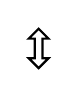
\begin{tikzpicture}
					% Draw a double-sided unfilled arrow, scaled down to one-quarter size
					\draw[thick] (0,0) -- (-0.125,0.125) -- (-0.05,0.125) -- (-0.05,0.375) -- (-0.125,0.375) -- (0,0.5) -- (0.125,0.375) -- (0.05,0.375) -- (0.05,0.125) -- (0.125,0.125) -- cycle;
				\end{tikzpicture}
				
			\end{center}
			%	\vspace*{-5pt}
			
			\begin{tikzpicture}
				\draw(0,0)
				to[short, -*](3.5,0) 
				to[short](4,0)
				to[short](4,0.5)
				to[R ,i ,v< , name =Ra  , l =$R_\mathrm{a}$] (4,2.5)
				to[short, i<_ , name = i0](4,3)
				to[short, -*](3.5,3)
				to[short](2,3)
				to[R ,i ,v< , name =R1  , l =$R_\mathrm{i}$]  (0,3)
				to[short](0,3)
				to[short, i<_ , name = i_0](0,2.5)  
				to[V, v, i, name=V1] (0,0.5)
				to[short](0,0); 
				
				\varrmore{R1}{$U_\mathrm{Ri}$};
				
				\varrmore{V1}{$U_0$};		
				\iarrmore{i0}{$I$};
				\draw[dashed] (-0.8,-0.3) -- (3,-0.3);
				\draw[dashed] (3,-0.3) -- (3,3.8);
				\draw[dashed] (3,3.8) -- (-0.8,3.8);
				\draw[dashed] (-0.8,3.8) -- (-0.8,-0.3);
				
				
				
				
				
			\end{tikzpicture}
			
			
			
			
		\end{columns}
		
		\speech{folie26}{1}{Abhängig vom Ziel der Netzwerkanalyse kann es sinnvoll sein, Stromquellen in Spannungsquellen oder Spannungsquellen in Stromquellen umzuwandeln.
			Dies funktioniert sowohl für reale Strom und Spannungsquellen als auch für Ersatzstrom beziehungsweise Ersatzspannungsquellen identisch. 
			Bei der Umwandlung bleibt der Wert des Innenwiderstandes R Ih erhalten. 
			Es ändert sich jedoch seine Position im Ersatzschaltbild. Die obere Abbildung stellt hierbei eine Ersatzstromquelle mit parallel geschaltetem Innenwiderstand dar, 
			die untere eine Ersatzspannungsquelle mit in Reihe geschaltetem Innenwiderstand.  
			Die Leerlaufspannung beziehungsweise der Kurzschlussstrom bleiben bei der Umwandlung der Quelle erhalten und werden mit Hilfe des Innenwiderstandes auf die jeweils andere Quelle umgerechnet.
			Als letzter Schritt bei der Quellenumwandlung müssen die Zählpfeile der Quelle noch umgedreht werden. Während der Zählpfeil von I null bei der Stromquelle nach oben zeigt, zeigt der Zählpfeil
			der äquivalenten Spannungsquelle in diesem Beispiel nach unten. 
		}
		\silence{4}
		
		
	}
\end{frame}



%\begin{frame}
%	\fta{Einfache Widerstandsnetzwerke}

%	\begin{Merksatz}{}


%	Bei der Reihenschaltung von Widerständen addieren sich die Werte der einzelnen Widerstände.
%	Der Strom durch alle in Reihe geschalteten Widerstände ist gleich. \\
%	Bei der Parallelschaltung berechnet sich der gesamte Leitwert aus der Summe der einzelnen Leitwerte.
%	Die Spannung an allen parallel gechalteten Widerständen ist gleich.
%	 \end{Merksatz}
%\end{frame}







%\begin{frame}
%    \fta{Kochrezept: Netzwerkanalyse}
%
%
%   \begin{columns}
%      \column[t]{0.5\textwidth}
%
%      \vspace*{-15pt}
%
%	  Liegt eine \textbf{Reihenschaltung} vor:
%	  \begin{enumerate}
%		\item Reihenschaltung wird von einem gemeinsamen Strom \(I\) durchflossen
%		\item Maschenumlauf aufstellen
%		\item Ohmsches Gesetz anwenden
%		\item Strom ausrechnen
%		\item Teilspannungen ausrechnen
%	\end{enumerate}
%
%	\vspace*{11pt}
%
%
%


%	  \begin{circuitikz}
%        \draw(0,0) to[short] (4,0)
%             to[R=$R_2$] (4,2)
%             to[R=$R_1$] (4,4)
%             to[short](0,4)
%			 to[V=$U_{1}$] (0,2)
%             to[V=$U_{2}$] (0,0);
%             \draw[->, blue] (4.5,3.5) -- (4.5,2.5) node[midway, right] {$U_\mathrm{R1}$};
%             \draw[->, blue] (4.5,1.5) -- (4.5,0.5) node[midway, right] {$U_\mathrm{R2}$};
%       \end{circuitikz}

%	   \begin{tikzpicture}
%       \draw(0,0) to[short] (4,0)
%           to[R=$R_2$,v<,name=R2] (4,2)
%          to[R=$R_1$,v<,name=R1] (4,4)
%         to[short](0,4)
%		 to[V,v,name=U1] (0,2)
%        to[V,v,name=U2] (0,0);
%
%			 \varrmore{R1}{$U_\mathrm{R1}$};
%			 \varrmore{R2}{$U_\mathrm{R2}$};
%			 \varrmore{U1}{$U_1$};
%			 \varrmore{U2}{$U_2$};
%      \end{tikzpicture}       
%
%      \column[c]{0.5\textwidth}
%
%		\pause
%
%		Liegt eine \textbf{Parallelschaltung} vor:
%
%		\begin{enumerate}
%			\item An allen Bauelementen der Parallelschaltung liegt dieselbe Spannung an
%			\item Knotengleichung aufstellen
%			\item Ohmsches Gesetz anwenden
%			\item Spannung ausrechnen%
%			\item Teilströme ausrechnen
%		\end{enumerate}
%
%


%		\begin{tikzpicture}
%           \draw(0,2)
%			to [short,i,name=in,o-]  (2,2)
%           to [R ,i>^ ,v , name =R1 ,*-* , l =$R_1$] (2 ,0)
%			to[short,i, name=out,-o](0,0);
%			\draw(2,2)
%			to [short,i]  (4,2)
%           to [R ,i>_ ,v , name =R2 ,*-* , l =$R_2$] (4 ,0)
%			to[short,i](2,0);	
%			\iarrmore{in}{$I_0$};
%			\iarrmore{R1}{$I_1$};
%			\iarrmore{R2}{$I_2$};
%			\iarrmore{out}{$I_3$};
%        \end{tikzpicture}


%	\begin{Merksatz}{}
%	Dies ist ein Merksatz .
%	\end{Merksatz}

%    \end{columns}

%\end{frame}
